\documentclass[11pt, a4paper]{article}
% Definition of title page:
\usepackage{graphicx, amsmath}
%\usepackage{amscd}
%\usepackage[tableposition=top]{caption}
%\usepackage{ifthen}
%\usepackage[utf8]{inputence}

\renewcommand{\theequation}{\arabic{section}.\arabic{equation}}
\textheight=9.4in \textwidth=15.2cm \oddsidemargin=.175in
\footskip=.3in \topmargin=-.2in
% \setlength{\oddsidemargin}{-.25in}
%\setlength{\textwidth}{6.5in} \setlength{\textheight}{10.5in}
%\setlength{\leftmargin}{-75in} \setlength{\evensidemargin}{-8in}
%\setlength{\parsep}{0.06 in} \setlength{\headheight}{0.5cm}
%\setlength{\topskip}{3pt} \setlength{\topmargin}{-0.3in}
%\setlength{\headsep}{0.05cm}
\renewcommand{\theequation}{\arabic{section}.\arabic{equation}}
\def\b#1{\mbox{\boldmath${#1}$}} %defines bold characters
\def\bmu{\mbox{\boldmath${\mu}$}} %defines bold \mu
\def\bdelta{\mbox{\boldmath${\delta}$}} %defines bold \delta
\def\bmuh{\mbox{\boldmath${\hat{\mu}}$}} %defines bold \delta\tilde
\def\bmut{\mbox{\boldmath${\tilde{\mu}}$}} %defines bold \delta\tilde
\def\btheta{\mbox{\boldmath$\theta$}} %defines bold \theta
\def\bbeta{\mbox{\boldmath$\beta$}} %defines bold \beta
\def\bSigma{\mbox{\boldmath$\Sigma$}} %defines bold \Sigma
\def\bGamma{\mbox{\boldmath$\Gamma$}} %defines bold \Gamma
\def\bb{\mbox{\boldmath$b$}} %defines bold b
\def\bB{\mbox{\boldmath$B$}} %defines bold B
\def\bS{\mbox{\boldmath$S$}} %defines bold S
\def\bR{\mbox{\boldmath$R$}} %defines bold R
\def\bE{\mbox{\boldmath$E$}} %defines bold E
\def\be{\mbox{\boldmath$e$}} %defines bold e
\def\bd{\mbox{\boldmath$d$}} %defines bold d
\def\bX{\mbox{\boldmath$X$}} %defines bold X
\def\bx{\mbox{\boldmath$x$}} %defines bold x
\def\bY{\mbox{\boldmath$Y$}} %defines bold Y
\def\by{\mbox{\boldmath$y$}} %defines bold y
\def\bZ{\mbox{\boldmath$Z$}} %defines bold Z
\def\bz{\mbox{\boldmath$z$}} %defines bold z
\def\bA{\mbox{\boldmath$A$}} %defines bold A
\def\bF{\mbox{\boldmath$F$}} %defines bold F
\def\bQ{\mbox{\boldmath$Q$}} %defines bold Q
\def\bl{\mbox{\boldmath$l$}} %defines bold l
\def\b0{\mbox{\boldmath$0$}} %defines bold 0
\def\bZ{\mbox{\boldmath$Z$}} %defines bold Z
\def\bt{\mbox{\boldmath$t$}} %defines bold t
\def\bI{\mbox{\boldmath$I$}} %defines bold I
\def\bee{\mbox{\boldmath$ee$}} %defines bold ee
\def\blambda{\mbox{\boldmath$\lambda$}} %defines bold \lambda
\def\bdelta{\mbox{\boldmath$\delta$}} %defines bold \delta

\title{\textbf{Risk factors for fouling biomass: Evidence from small vessels in Australia}}
%#\author{Md. Enamul Kabir\footnote{on leave from Department of Statistics, University of Dhaka, Bangladesh.}\ and Shahjahan Khan\\
%#Department of Mathematics \& Computing\\
%#Australian Centre for Sustainable Catchments\\
%#University of Southern Queensland\\
%#Toowoomba, Qld 4350, AUSTRALIA\\
%#\em{Emails: kabir@usq.edu.au} \rm{and} \em{khans@usq.edu.au}}
\date{}
\begin{document}
\maketitle

\begin{abstract}


This paper applies statistical methods to investigate the potential risk factors for fouling biomass of small vessels. The results are examined in order to identify the factors that can help vessels owner for reducing to corrosion of the vessels and to a increase in the efficiency of moving parts. \\

\end{abstract}


\section{Introduction}


Biofouling is a process where organisms accumulate on a clean surface that has been immersed in the marine environment. Biofouling on vessel hulls thus provides a means by which organisms can be transferred to new locations.



The human-mediated introduction of non-indigenous marine species into new locations can have catastrophic ecological, economic and social consequences (Carlton 1996, 2001; Pimentel et al. 2000; Hewitt 2003). For example, associated damages and costs of controlling aquatic invaders in the United States are estimated to be US \$9 billion annually (Pimentel et al. 2000).


The movement of vessels has been identified as the single most important vector for the dispersal of non-indigenous marine species around the world.  For the past three decades, ballast water discharges from commercial vessels were thought to be the most significant mechanism for the dispersal of non-indigenous marine species, however recent research suggests that more non-indigenous marine species introductions are attributable to vessel biofouling than any other mechanism (Hewitt et al. 1999, 2004; Mineur et al. 2007).
A risk assessment to identify and determine the quarantine risk to Australia associated with the entry, establishment and spread of marine pest species as biofouling has been conducted. The Species biofouling risk assessment (SBRA) (Hewitt et al. 2011), assessed over 1781 marine and estuarine species that have been introduced into areas outside their natural range. The SBRA identified 56 species of concern (SOC) that are not currently known to be present in Australia, have a high probability of arriving in Australian waters as biofouling on international vessels and have the potential to cause unacceptable impacts to environmental, economic, social/cultural or human health values.




\section{Materials and methods}


The data used in this paper came from a prospective survey in Australia conducted by the Commonwealth Scientific and Industrial Research Organisation (CSIRO) project team. The team sampled $54$ vessels at $5$ locations during the project. Most vessels were sampled in Hobart at the Domain Slipway ($16$) and Royal Hobart Yacht Club ($18$). The remaining vessels were sampled in Melbourne at the Sandringham Yacht Club ($14$), the Hobson's Bay Yacht Club ($4$) and the Royal Yacht Club of Victoria ($2$). Most of the sample vessels were yachts ($32$), followed by fishing vessels ($10$) and motor cruisers ($10$). The project team also sampled a ferry and a tug. The team inspected $64$ different locations in and around the hull, propeller, rudder and anchor, internal spaces, fishing gear and deck of the sample vessels. $1116$ samples were taken mainly from the hull. A further $365$ inspections were made on board. The wet weight of fouling biomass is taken from each sample. The samples containing weight $\leq 0.5$ grams or less were assumed to contain no biomass and were regarded as clean samples. The response variable is the wet weight of fouling biomass and is treated as a binary variable by assigning the value $'0'$ signifying 'clean samples' and the value $'1'$ signifying the event of having biomass. The predictor variables are the number of days since the vessel was last used (days1), the number of days since the vessel was last cleaned (days2), median number of trips per year (midTrips) and the qualitative predictor (paint type) with three levels (ablative, hard and self-polishing).\\


Various statistical methods are used in this study to analyse the data on fouling biomass in Australia. The first method is based on the application of Generalized linear mixed-effects model (GLMM) to identify the factors that are associated with biomass. The GLMM is considered considering boatID as a random effect as there seems to be evidence that there are correlation/similarities among observations within same boat. In the interests of expediency, GLMM is fitted in the nine locations, namely fixed keel (HP), the boot-top (HAH), depth sounder booth (HH), water inlet/outlet cover plates (HD), propeller surface (PB), rudder surface (PJ), hull quadrats (HA), seawater/grey water inlets/outlets (IB) and paddle wheel and booth (HK). There may be a case that the relationship between the variables is expected to be of a complex form and not easily fitted by standard linear or non-linear models. Generalized additive model (GAM) do not involve strong assumptions about the relationship that is implicit in standard parametic regression. Infact, such assumptions may force the fitted relationship away from its natural path at critical points. Thus we use a Generalized additive mixed-effect model (GAMM) considering $b$-splines of days1 and days2 and we use thin plate regression and cubic splines respectively.\\

The wet weight fouling biomass of non-zero samples is approximately log-distributed. In this scenario, Linear regression model (LRM) is not appropriate as it ignores possible boat specific effects, i.e., correlation among observations within a boat. Thus we fit a LMM to show the relation between non-zero biomass and a set of explanatory variables, namely days1, days2, midTrips and paitType. It should be noted that the hull quadrats (HA) provide the basis for much of this modeling because the sample ares (0.5m$^2$) in each case is held constant and therefore comparable between vessels. In most other instances the sample area is determined by the size of the relevant location (e.g., water inlet/outlets, transducer) and therefore varies between vessels. Therefore, for this modeling we only consider non-zero biomass collected from HA. There is no guarantee that the relationship between the response variable and the continuous predictors should be linear, in fact, such a claim would tend to lack credibility. We need a model that will permit the detection of curvature, but not enforce it. Thus we again fit a GAMM model considering smooths of days1 and days2 and the parametric term of other variables. In all of these cases, the classical ANOFA (F-test) and parametric bootstrap (TP) test is considered to choose the best-predicted model from among all selected variables.

\section{Graphical summary and data exploration}

Figure \ref{scatter} shows scatter plot matrix, the histograms on the diagonal and the correlation coefficients in the upper triangle. The figure shows that there seems to be some outliers in the data. However, it does not seem any pairwise correlation among the variables. Thus for further analysis, we will keep all four variables.


\begin{figure}
\centering
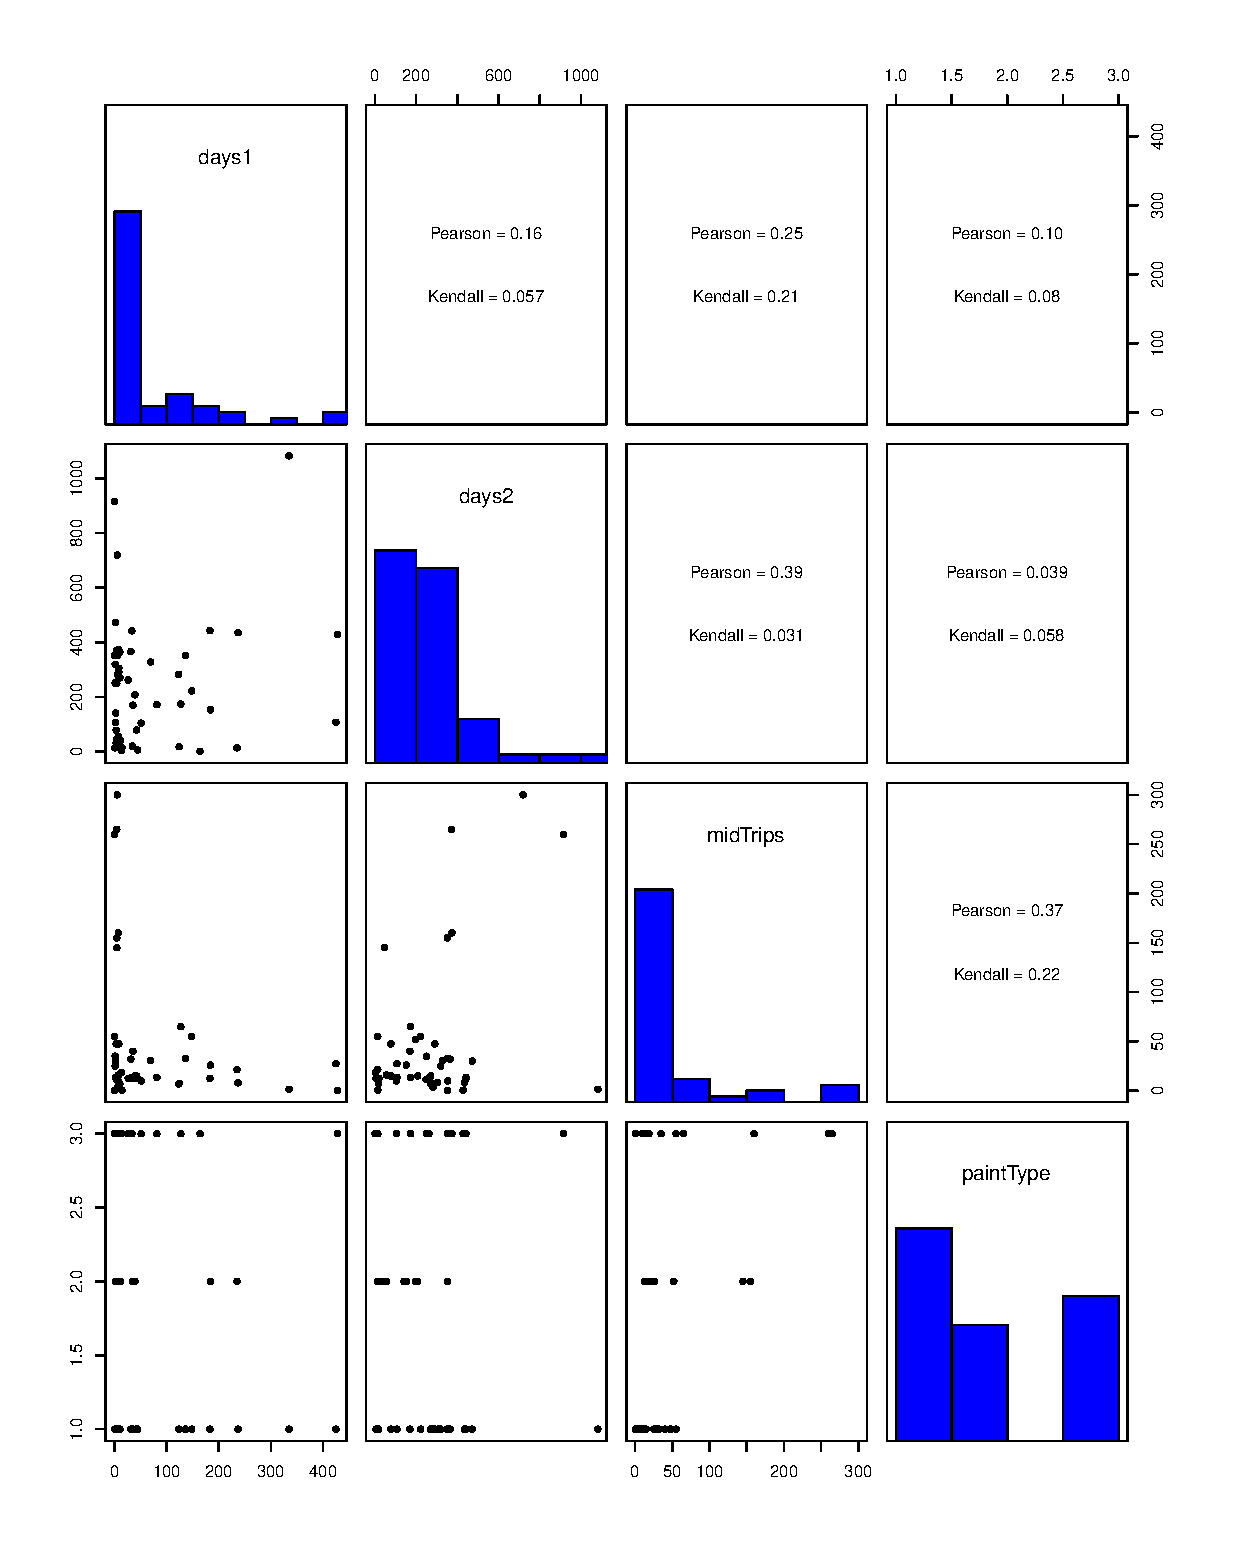
\includegraphics[scale=.7]{../graphics/scatter.eps}
\caption{Scatter plot matrix, the histograms on the diagonal and the correlation coefficients in the upper triangle} \label{scatter}
\end{figure}

Figure \ref{histogram}shows histograms of sample wet weight (grams) for the whole sample (a), the log of sample wet weight (grams) for the whole sample (b), sample wet weight (grams) for the non-zero (biomass) sample (c), and the log of sample wet weight (grams) for the non-zero (biomass) samples (d). Histogram of wet weight (grams) shows that samples are zero-inflated. However, histogram of log transformed data shows that samples are approximately normally distributed. On the other hand, the wet weight fouling biomass of non-zero samples is approximately log normally distributed but the log of these non-zero biomasses is normally distributed.



\begin{figure}
\centering
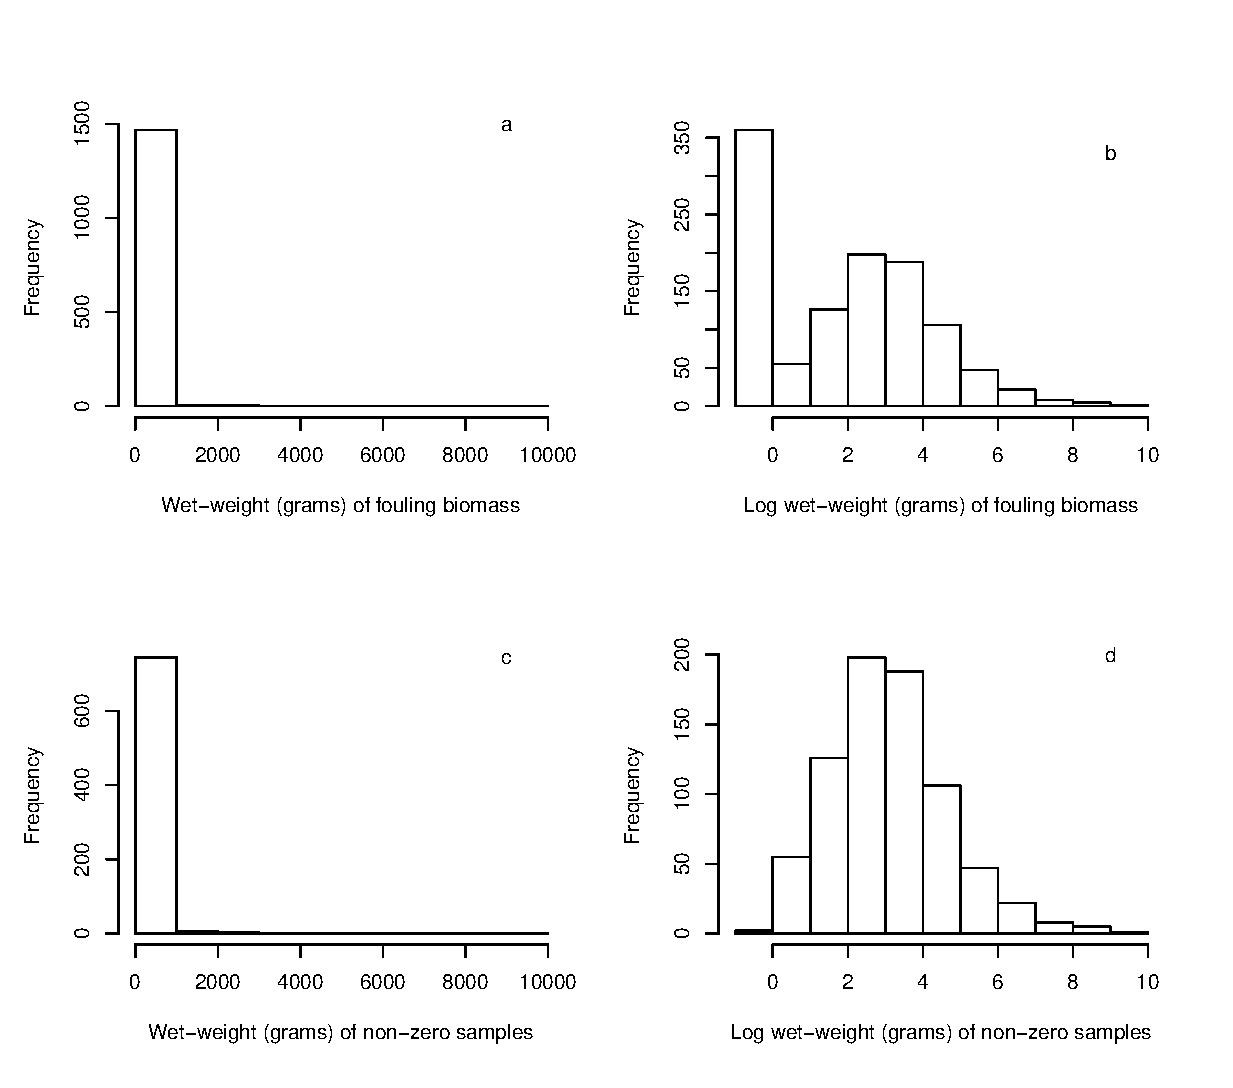
\includegraphics[scale=.7]{../graphics/histogram.eps}
\caption{Histograms of sample wet weights (grams)} \label{histogram}
\end{figure}


These smooth plots in figure \ref{smooth} show that there is a variation of log of the wet-weight (grams) among the levels of paint-type factor. The smooth plots also show there is a variation of log of the wet-weight among different LocID.


\begin{figure}
\centering
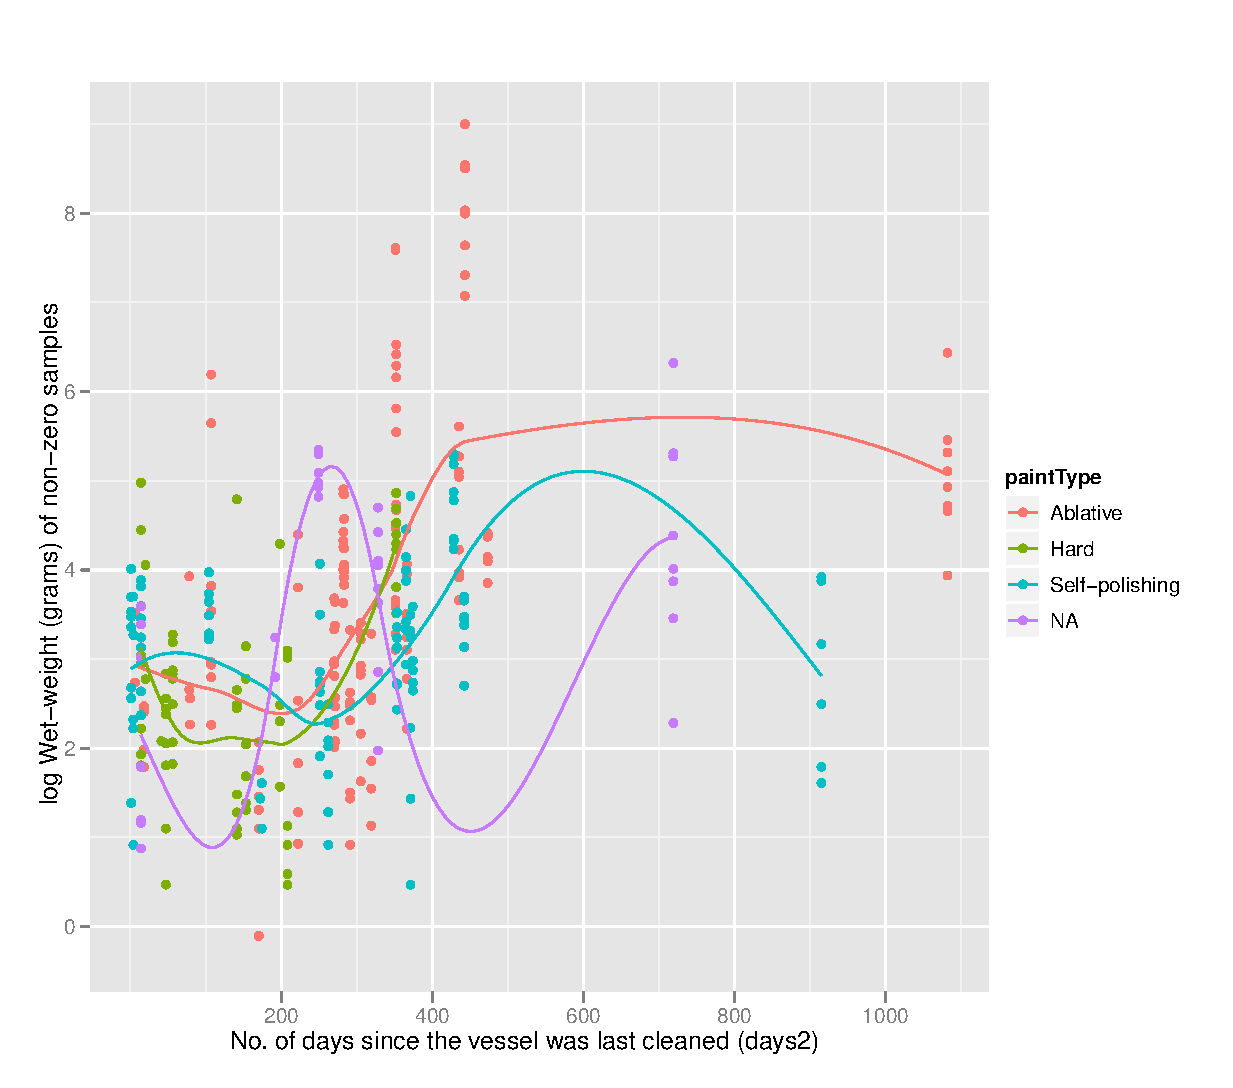
\includegraphics[width=0.43500\textwidth]{../graphics/1.eps}  %\hspace{00cm}
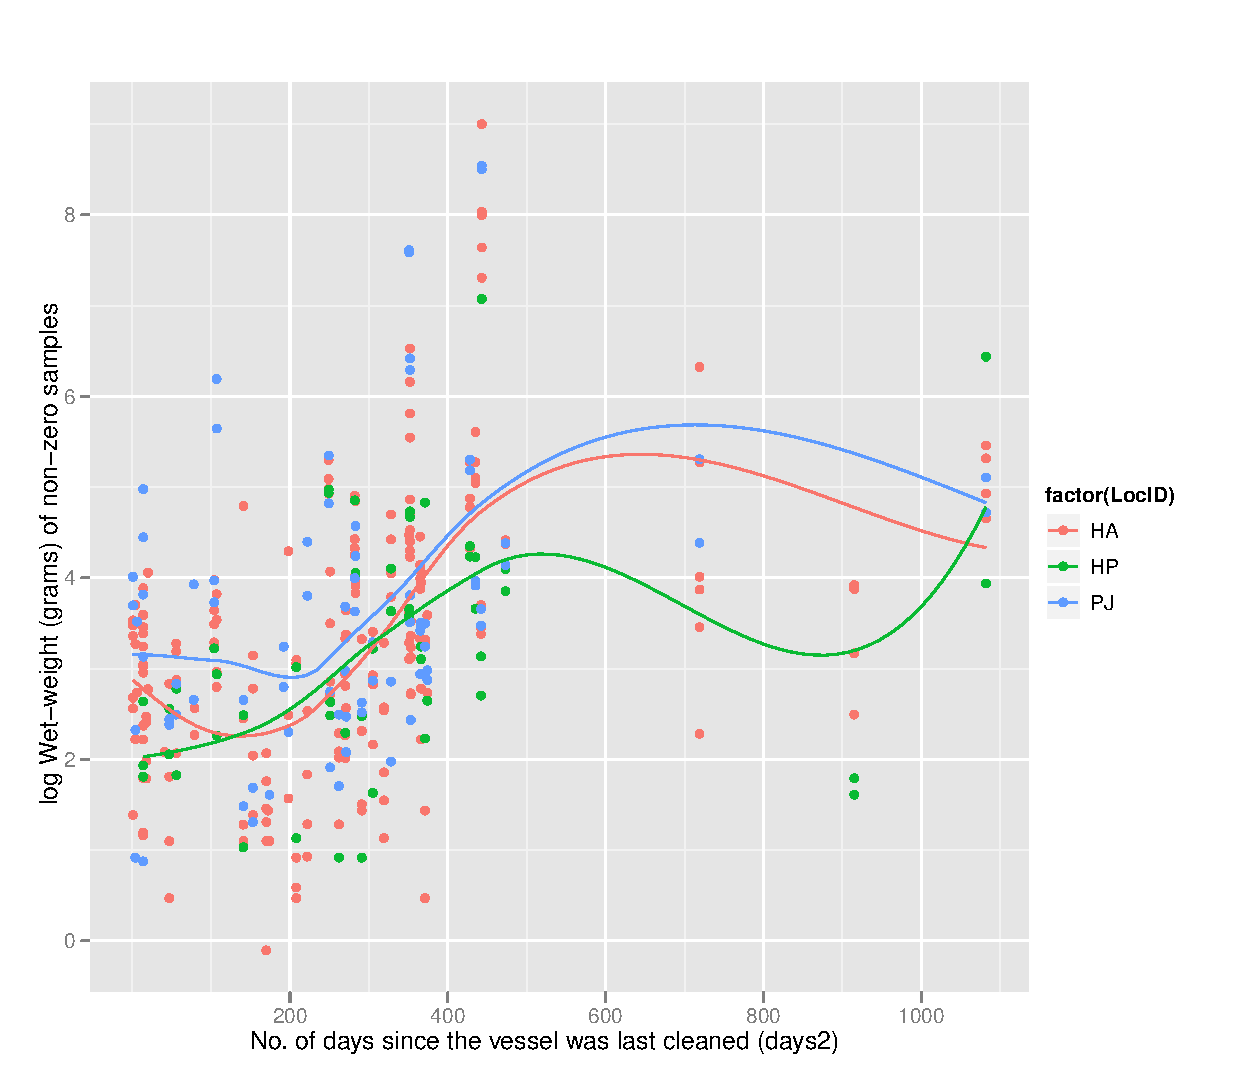
\includegraphics[width=0.43500\textwidth]{../graphics/2.eps} %\vspace{00cm}
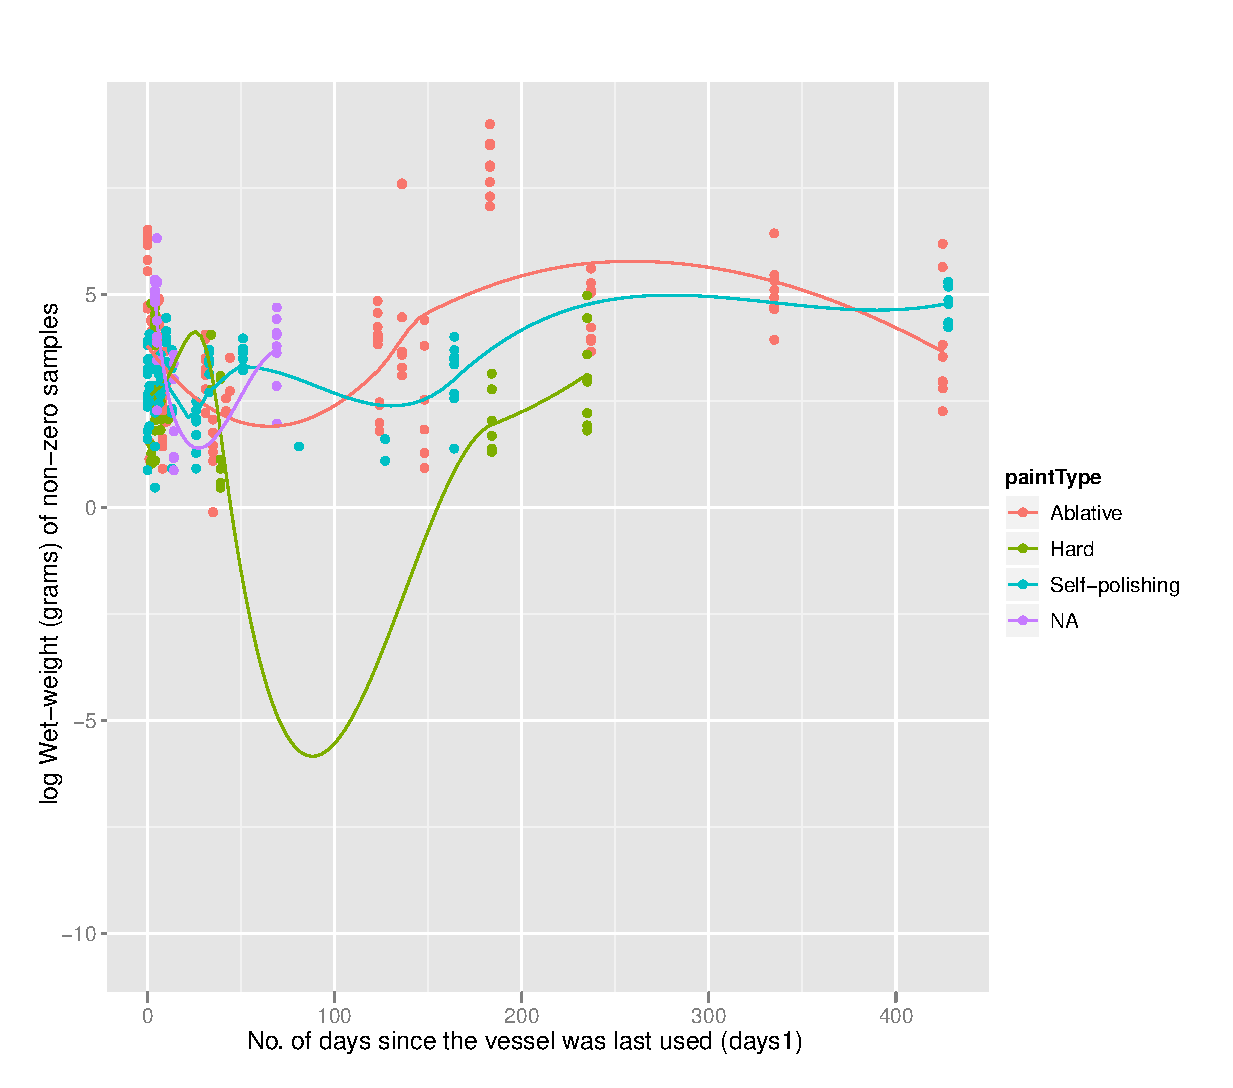
\includegraphics[width=0.43500\textwidth]{../graphics/3.eps} %\hspace{00cm}
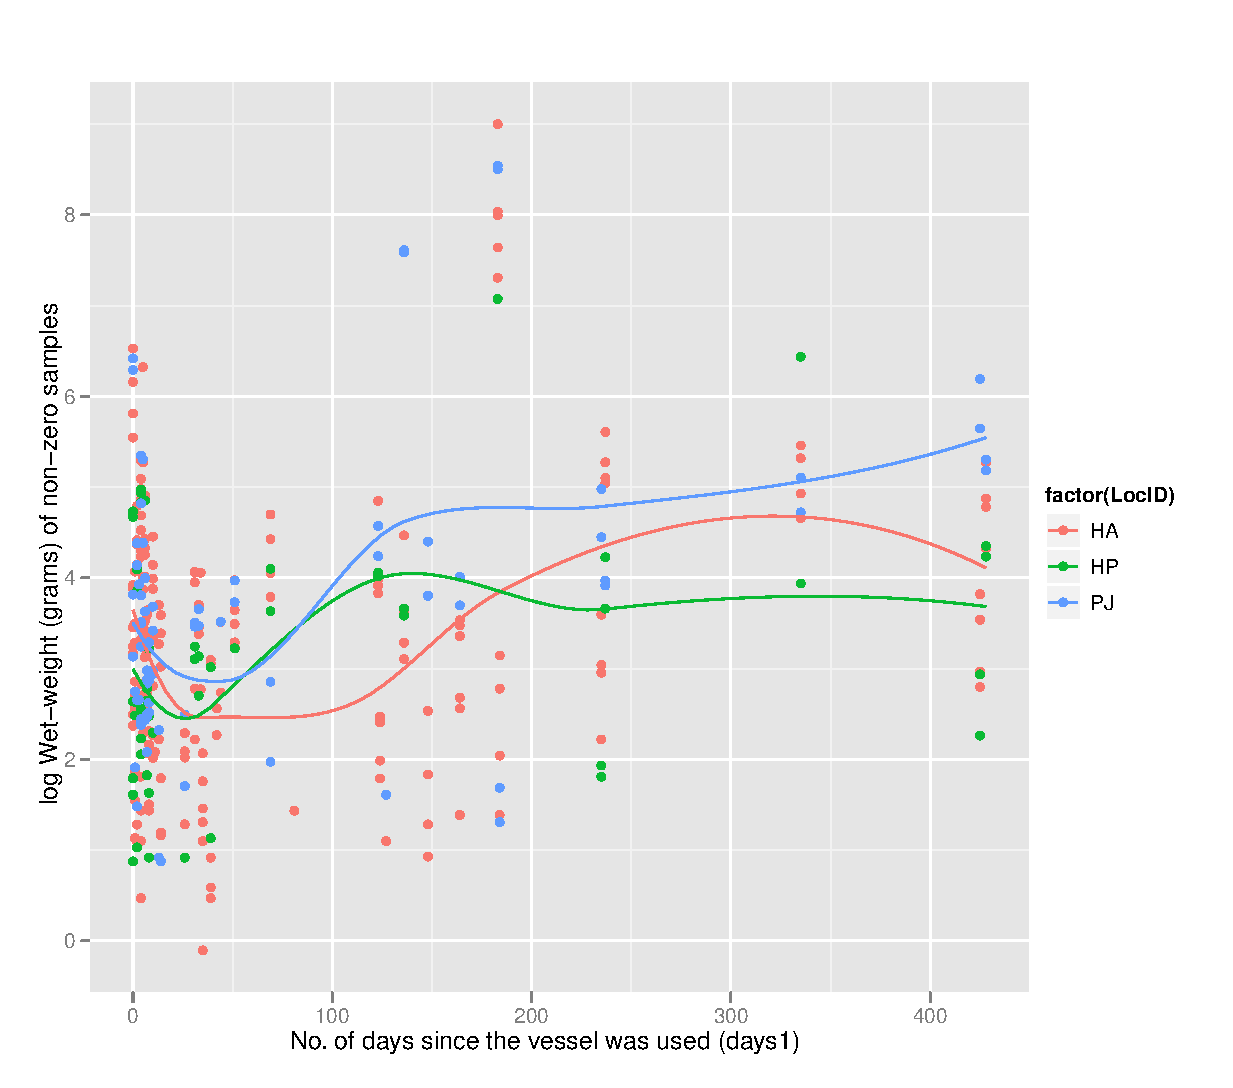
\includegraphics[width=0.43500\textwidth]{../graphics/4.eps} %\vspace{00cm}
%\includegraphics[width=0.3500\textwidth]{all_power_alpha_.10_delta_0_sigma.eps} %\hspace{00cm}
%\includegraphics[width=0.3500\textwidth]{all_power_alpha_.10_delta_0_nsigma.eps} %\vspace{00cm}
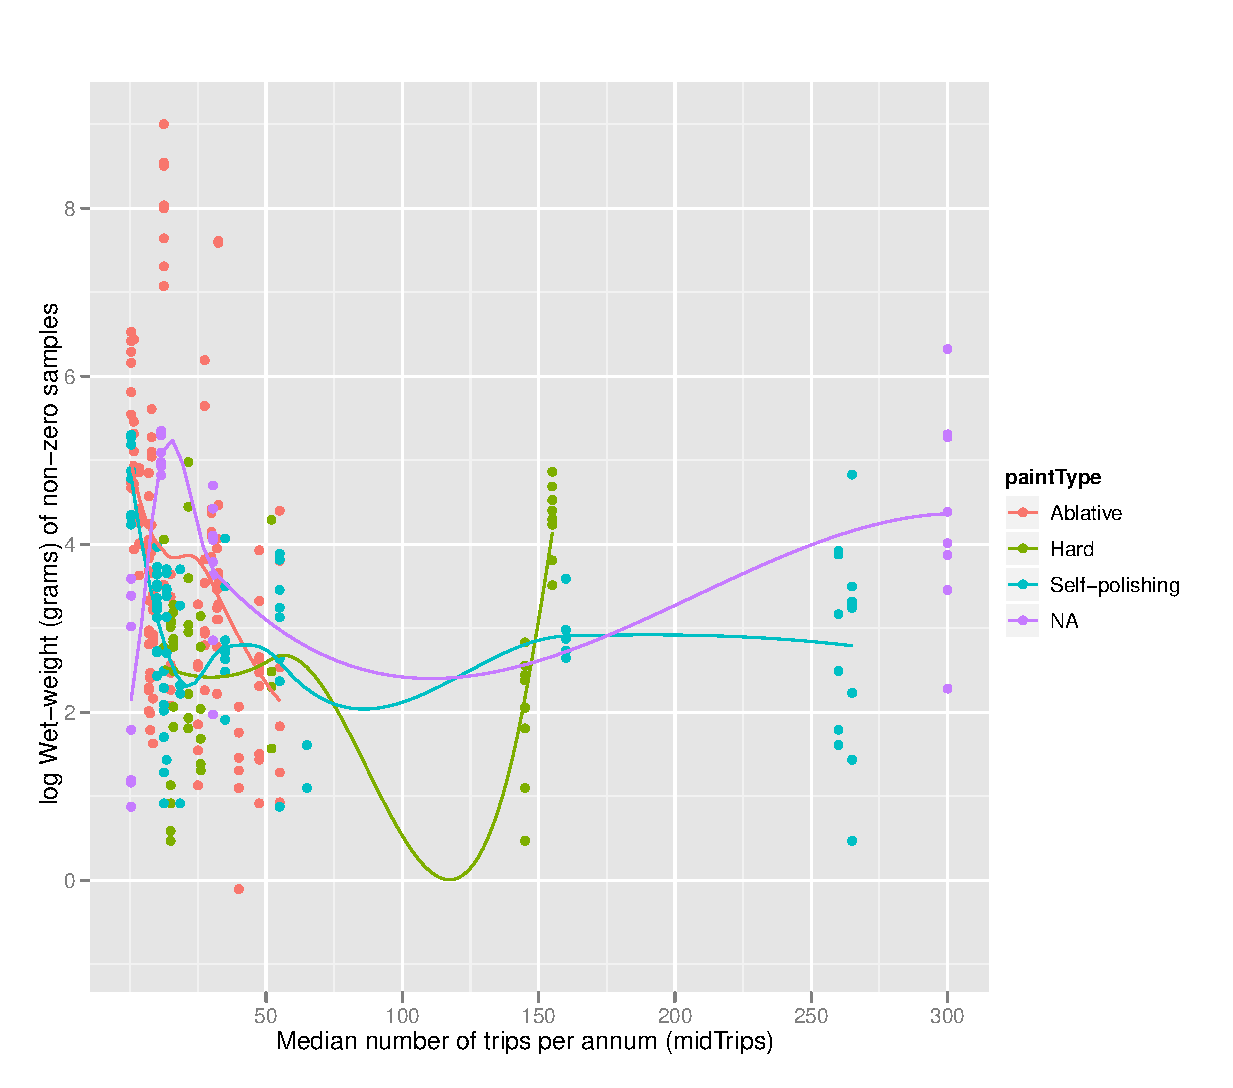
\includegraphics[width=0.43500\textwidth]{../graphics/5.eps}  %\hspace{00cm}
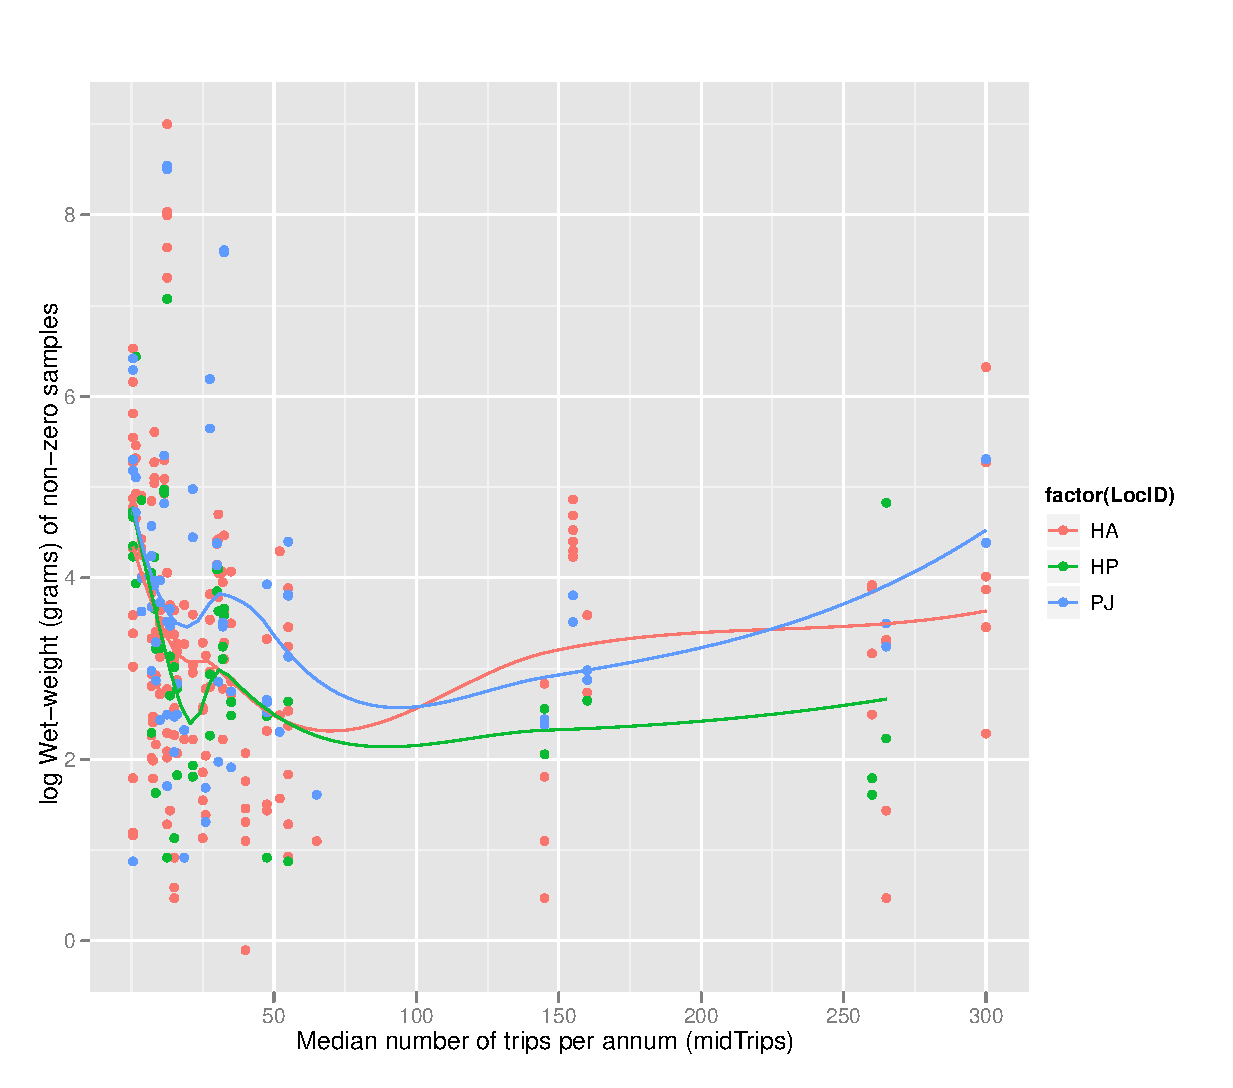
\includegraphics[width=0.43500\textwidth]{../graphics/6.eps} %\vspace{00cm}
\caption{Smooth plots showing the log of the wet weight (grams) of biomass among the levels of paint type and LocID against days1, days2 and midTrips.}
\label{smooth}
\end{figure}


Figure \ref{boxplot} shows box plot of log of the non-zero sample weights (grams) against location ID (LocID).


\begin{figure}
\centering
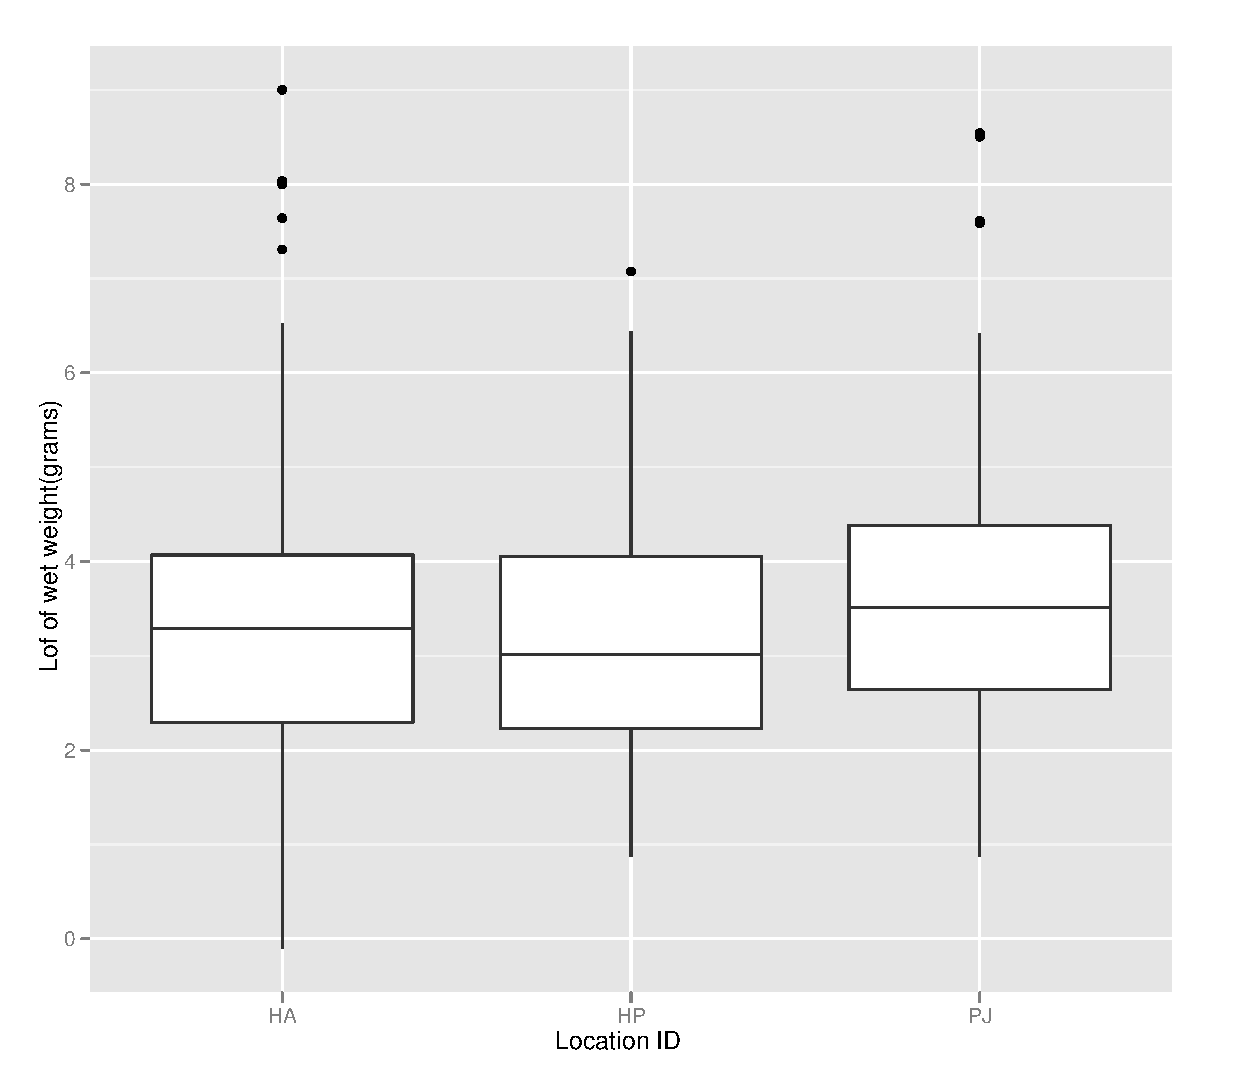
\includegraphics[scale=.7]{../graphics/boxplot.eps}
\caption{Box plot of log of non-zero sample wet weights (grams)} \label{boxplot}
\end{figure}




From Figure \ref{propzero} suggests that days1 and midTrips have very little predictive power in this context. In this initial inspection the predictive power of days2 appeared to be more promising. Repeating this analysis with standard sampling units doesn't change the message. Our initial deduction is also supported by the quasi likelihood analysis that the predictive power of days2 is more convincing as days2 is statistically significant for the proportion of non-zero samples ($p$-value=1.9$\times 5e^{-12}$).

\begin{figure}
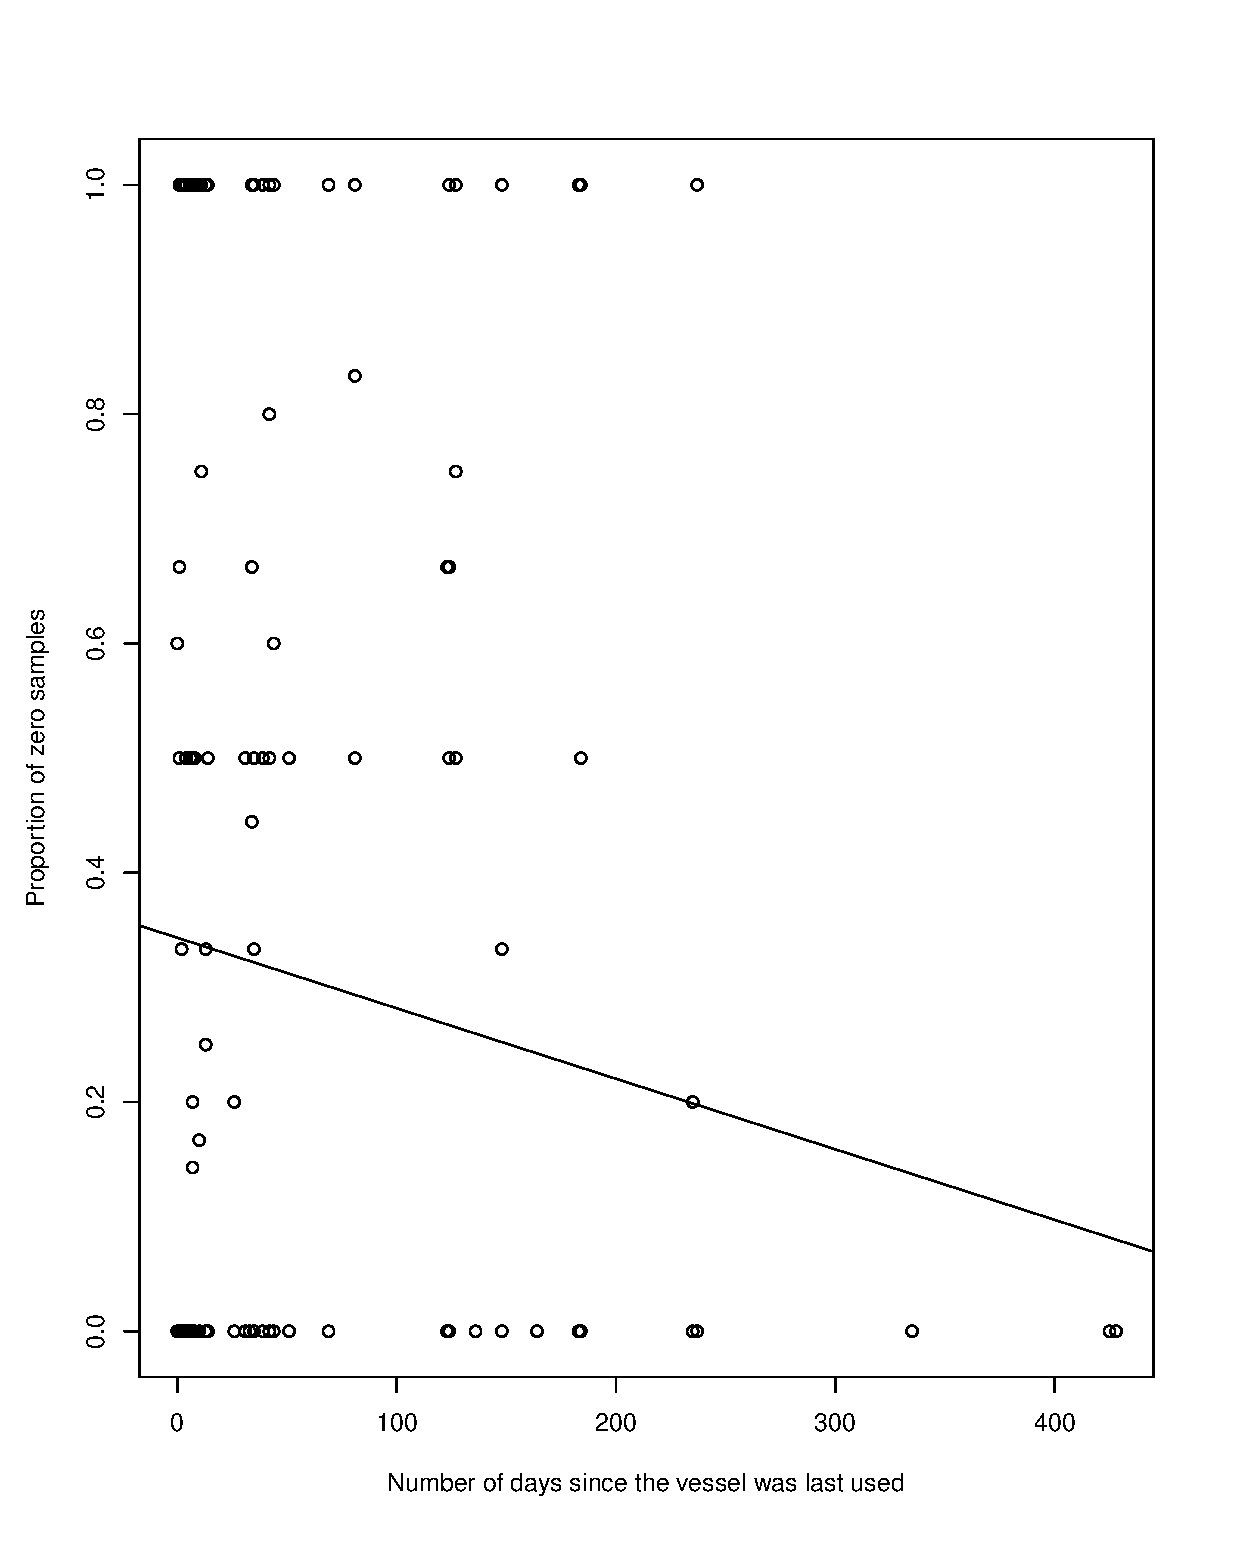
\includegraphics[width=0.3\textwidth]{../graphics/propzerodays1.eps}
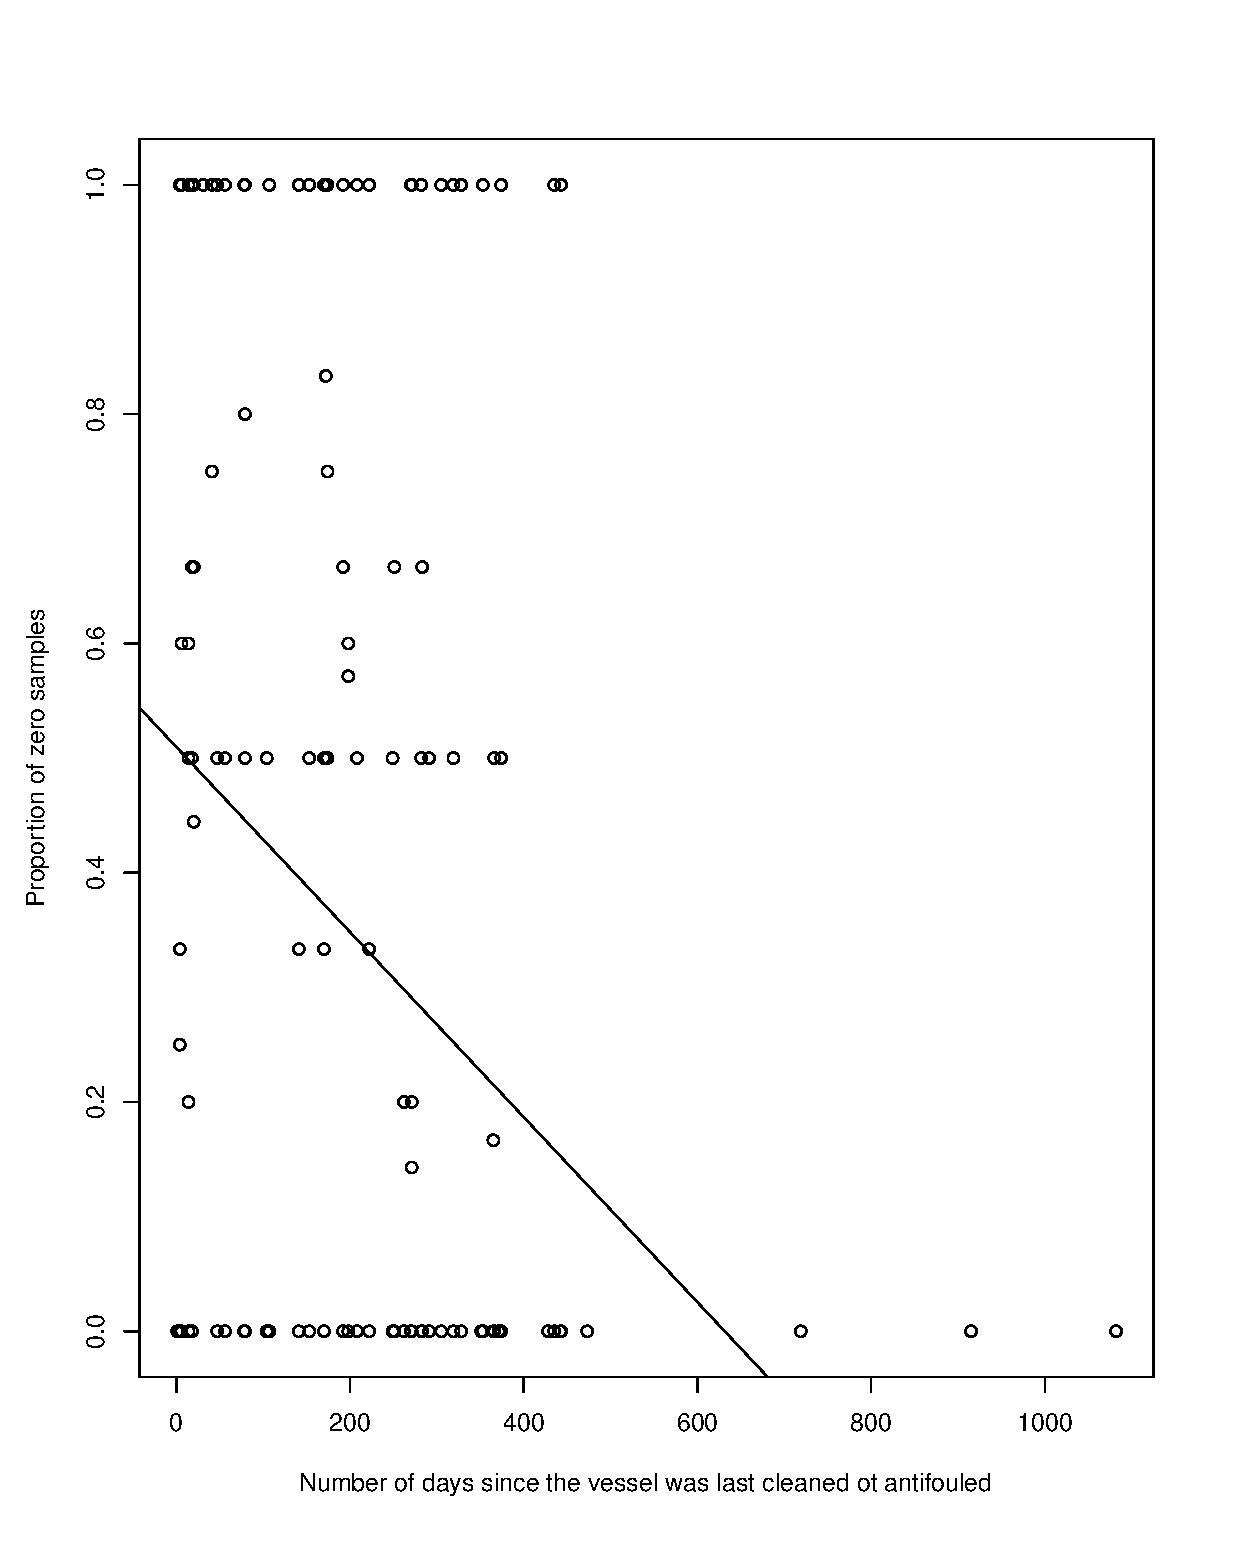
\includegraphics[width=0.3\textwidth]{../graphics/propzerodays2.eps}
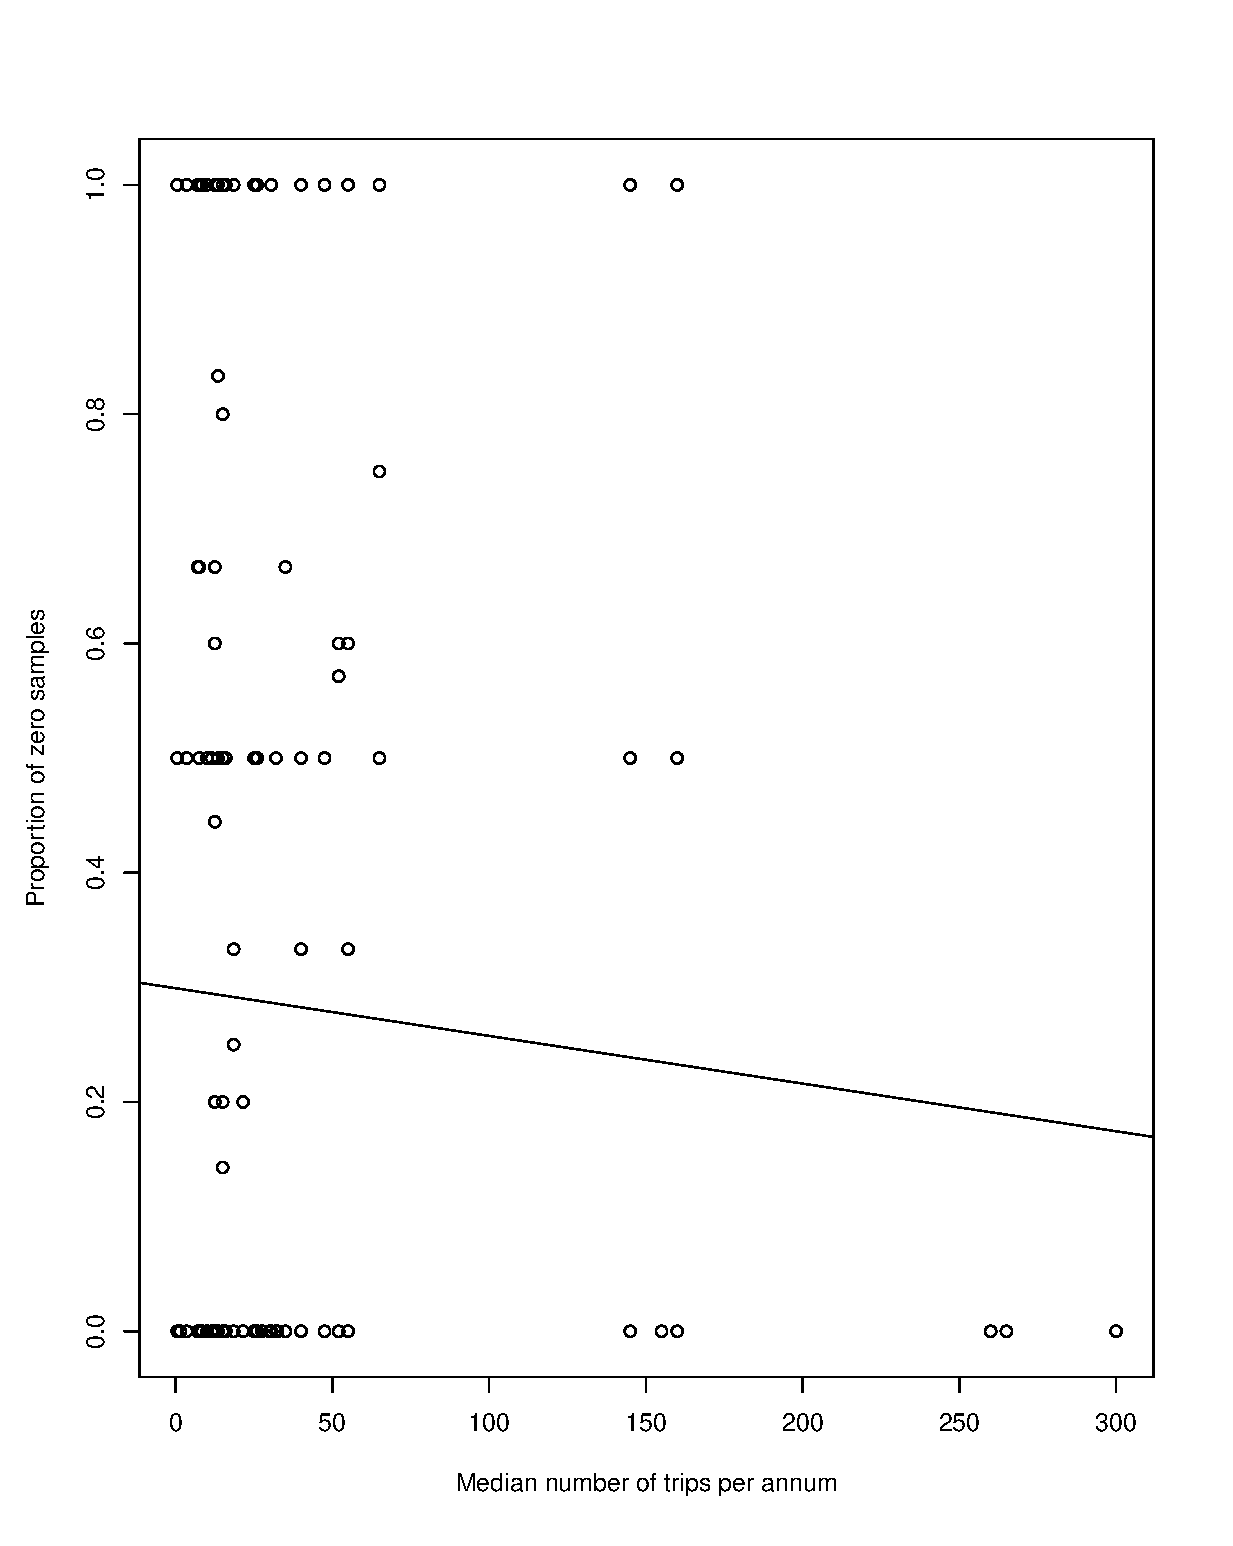
\includegraphics[width=0.3\textwidth]{../graphics/propzeromidTrips.eps}
\caption{Relationship between the proportions of zero samples in each location and the three potential explanatory variables, days1, days2 and midTrips.}
\label{propzero}
\end{figure}




Figure \ref{prezerodays2} shows Actual and predicted proportion of zero samples based on quasi-likelihood analysis against the number of days since the vessel was last cleaned. The graph shows that the proportion of clean samples diminishes very quickly after vessel has been clean or antifouled. If we remove the three vessels where days2 more than 600 days, we get very similar results.

\begin{figure}
\centering
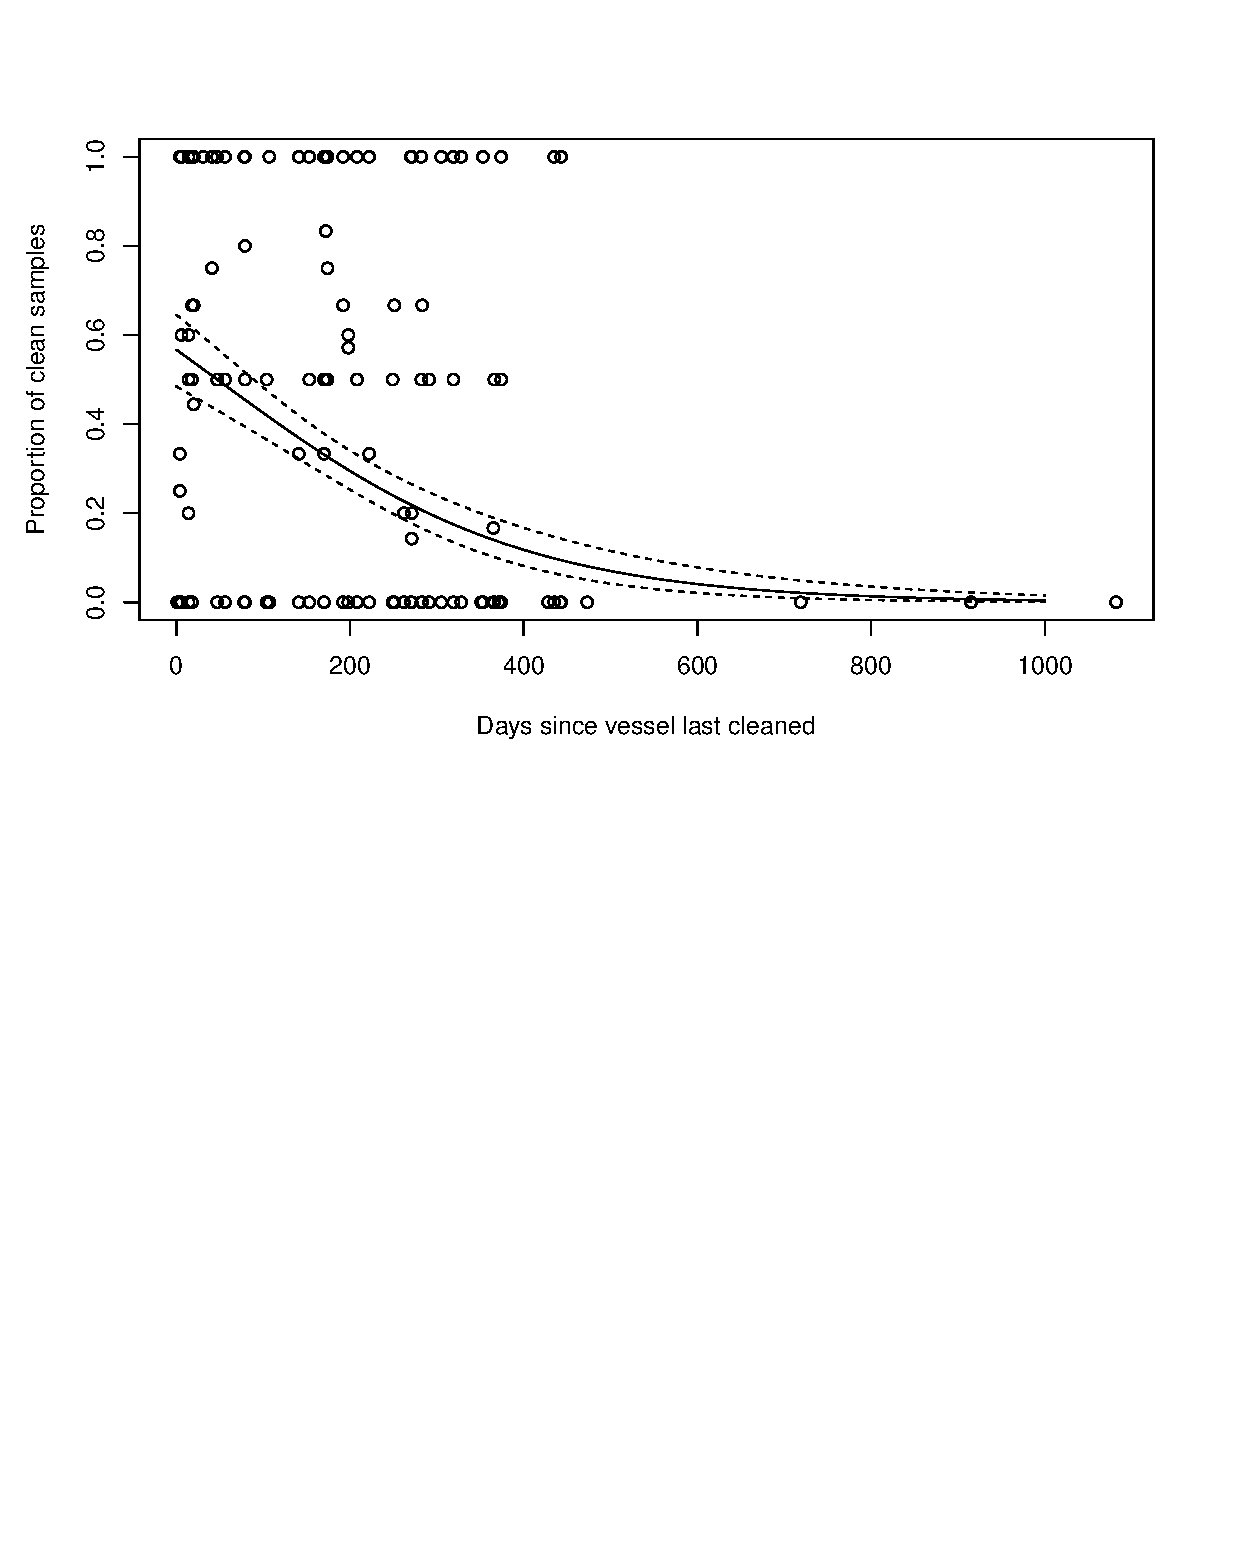
\includegraphics[scale=.7]{../graphics/prezerodays2.eps}
\caption{Actual and predicted proportion of zero samples based on quasi-likelihood analysis.} \label{prezerodays2}
\end{figure}









\section{Results}

\hspace{-6mm}\underline{Generalized linear mixed-effect model (GLMM)}\\

As mentioned before, for determining the real influencing factors of biomass (i.e., to identify the determinants of biomass), a multivariate logistic regression analysis can be performed, considering four influencing factors (days1, days2, midTrips, paintType) as well as their interactions. However, MLR analysis ignores possible boat specific effects, i.e., correlation among observations within a boat as there seems to be evidence that there are correlation/similarities among observations within same boat. This should not be too surprising: presumably there are many characteristics of the boats that affect biomass, beyond what we are including in the model. To address this question, we need to fit a model which allows for such effects. To keep it simple, we consider a model with just a random intercept for each boat. We could in principle include random slope terms, but keep in mind we only may have some observations for small observations for some boat. So there is any limited information about any boat-specific effects at all. The generalized linear mixed-effect model (GLMM) is a natural match in this situation. First we fit a model considering binary response of biomass (1, if biomass, 0 otherwise) and the predictors (days1, days2, midTrips, LocID, paitType) and their interactions.\\
\begin{small}
\begin{table}
%\begin{center}
\caption{Parameter estimates for Generalized linear mixed model fit by the Laplace approximation } \label{tab1}
\begin{tabular}{|c|c|c|c|c|} \hline
Fixed effects:                      &Estimate &Std. Error &z value &Pr($>|z|$)\\
\hline
(Intercept)                         &-1.8490863 &0.4623099 &-4.000 &6.34e-05 ***\\
days1                               &0.0178767  &0.0038331 &4.664  &3.11e-06 ***\\
days2                               &0.0141527  &0.0018132 &7.806  &5.92e-15 ***\\
paintTypeHard                       &2.0255413  &0.7127035 &2.842  &0.004482 ** \\
paintTypeSelf-polishing             &3.2006003  &0.6228237 &5.139  &2.76e-07 ***\\
factor(LocID)HAH                    &0.3626283  &0.5888398 &0.616  &0.538003 \, \, \,\\
factor(LocID)HD                     &-1.7557879 &0.4341652 &-4.044 &5.25e-05 ***\\
factor(LocID)HH                     &-0.4662680 &0.5493467 &-0.849 &0.396010 \, \, \,\\
factor(LocID)HK                     &-2.0871967 &0.5445139 &-3.833 &0.000127 ***\\
factor(LocID)HP                     &-0.7306755 &0.4307227 &-1.696 &0.089811 .\, \,\\
factor(LocID)IB                     &-1.2600510 &0.3191204 &-3.949 &7.86e-05 ***\\
factor(LocID)PB                     &-1.0067152 &0.4744011 &-2.122 &0.033831 *\, \, \,\\
factor(LocID)PJ                     &0.1945601  &0.4341810 &0.448  &0.654075 \, \, \,\\
days1:midTrips                      &-0.0003729 &0.0000931 &-4.006 &6.18e-05 ***\\
days1:paintTypeHard                 &-0.0009644 &0.0048503 &-0.199 &0.842392 \, \, \,\\
days1:paintTypeSelf-polishing       &-0.0179081 &0.0044233 &-4.049 &5.15e-05 ***\\
days2:paintTypeHard                 &-0.0052131 &0.0037719 &-1.382 &0.166939 \, \, \,\\
days2:paintTypeSelf-polishing       &-0.0100362 &0.0025790 &-3.892 &9.96e-05 ***\\
paintTypeHard:midTrips              &0.0060892  &0.0057800 &1.053  &0.292113 \, \, \,\\
paintTypeSelf-polishing:midTrips    &-0.0019841 &0.0039590 &-0.501 &0.616266 \, \, \,\\
\hline
\end{tabular}
\\

Signif. codes: \quad 0 �***� \quad 0.001 �**� \quad 0.01 �*� \quad 0.05 �.� \quad 0.1 \quad � � 1
%\end{center}
\end{table}
\end{small}

The summary of full model suggests dropping days2:midTrips. Refitting without this term, and then examining the significance of terms using both F-test and PB-test in the resulting model, suggests dropping midTrips. Continuing in the same, we select the best model which consists of the variables, days1, days2, paintType, LocID, days1:midTrips, days1:paintType, days2:paintType and midTrips:paintType. The results are presented in Table \ref{tab1}.GLMM is used to assess the independent effect of a variable on biomass after allowing for other variables that might have an influence on the underlying relationship. The results are presented in Table \ref{tab1} in the form of estimate, standard error, $z$-value and significant levels. GLMM suggests revealed that the probability of biomass of a vessel is  $1.014253$ $(e^{0.0141527})$ times higher for each day that the vessel is not cleaned. On the other hand, this probability is 1.018037 times higher for each day if the vessel is not used. Vessels that are painted by hard are 7.6 times more likely to be biomass than ablative paint and self-polishing are 24.5 times more likely to be biomass than its ablative counterparts.\\


GLMM also suggests that water inlet/outlet cover plates (HD), paddle wheel and booth (HK) and seawater/grey water inlets/outlets (IB) are respectively 83\%, 88\% and 72\% less likely to be biomass than the hull quadrats (HA). \\

\begin{figure}[h]
\centering
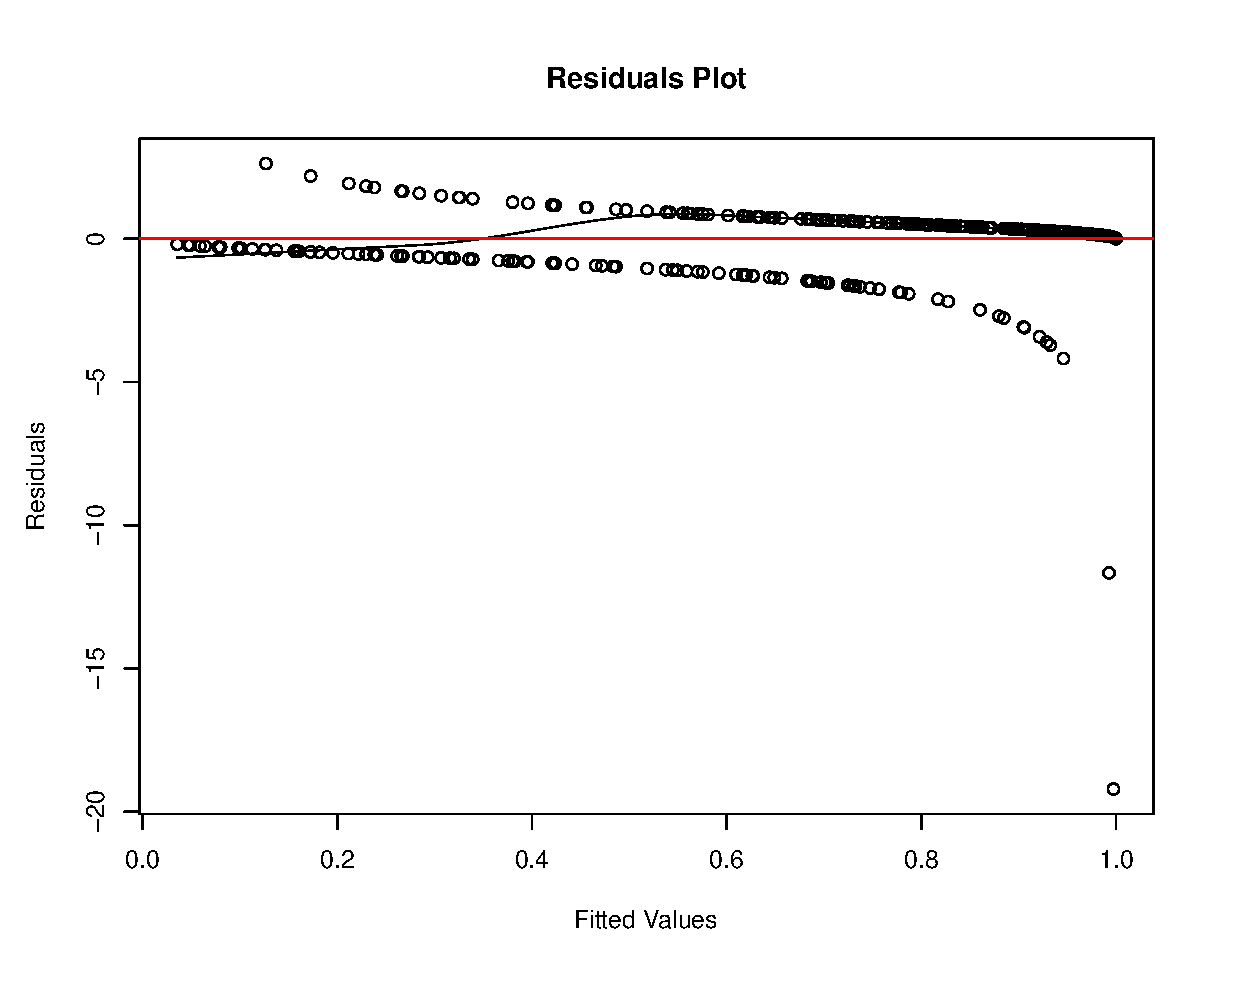
\includegraphics[width=0.50\textwidth]{../graphics/fig1.eps}  %\hspace{00cm}
\caption{ Residuals plot for the final GLMM model} %\vspace{1.05cm}
\label{fig1}
\end{figure}


\textbf{Residuals plot, Q-Q plot for residuals and Q-Q plot for boat effect of GLMM}\\


The residuals plot, Q-Q plot for residuals and Q-Q plot for random effects of the GLMM are shown respectively as in Figure \ref{fig1}, Figure \ref{fig2} and in Figure \ref{fig3}. The residual shows that there are some outliers. There is a curved pattern that indicates the residuals are non-linear.

  \begin{figure}
\centering
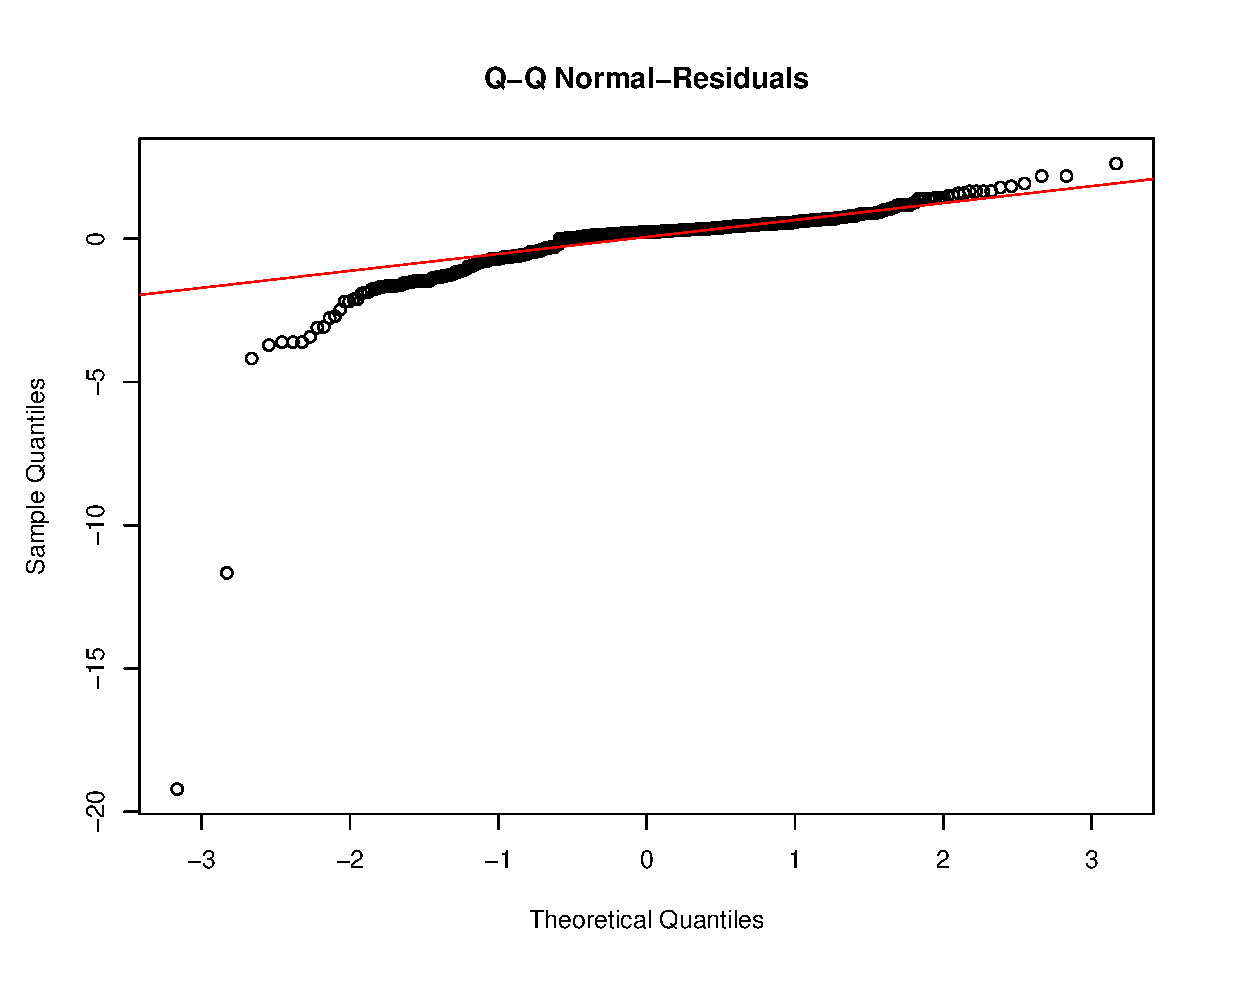
\includegraphics[width=0.50\textwidth]{../graphics/fig2.eps}  %\hspace{00cm}
\caption{ Q-Q plot for residuals of the final GLMM model} %\vspace{1.05cm}
\label{fig2}
\end{figure}

Q-Q plot for residual shows with the Gaussian assumption. Q-Q plot for random intercept for the final model looks good. Thus the gaussian assumption is satisfied, indicates that the final model is more reasonable.\\

  \begin{figure}
\centering
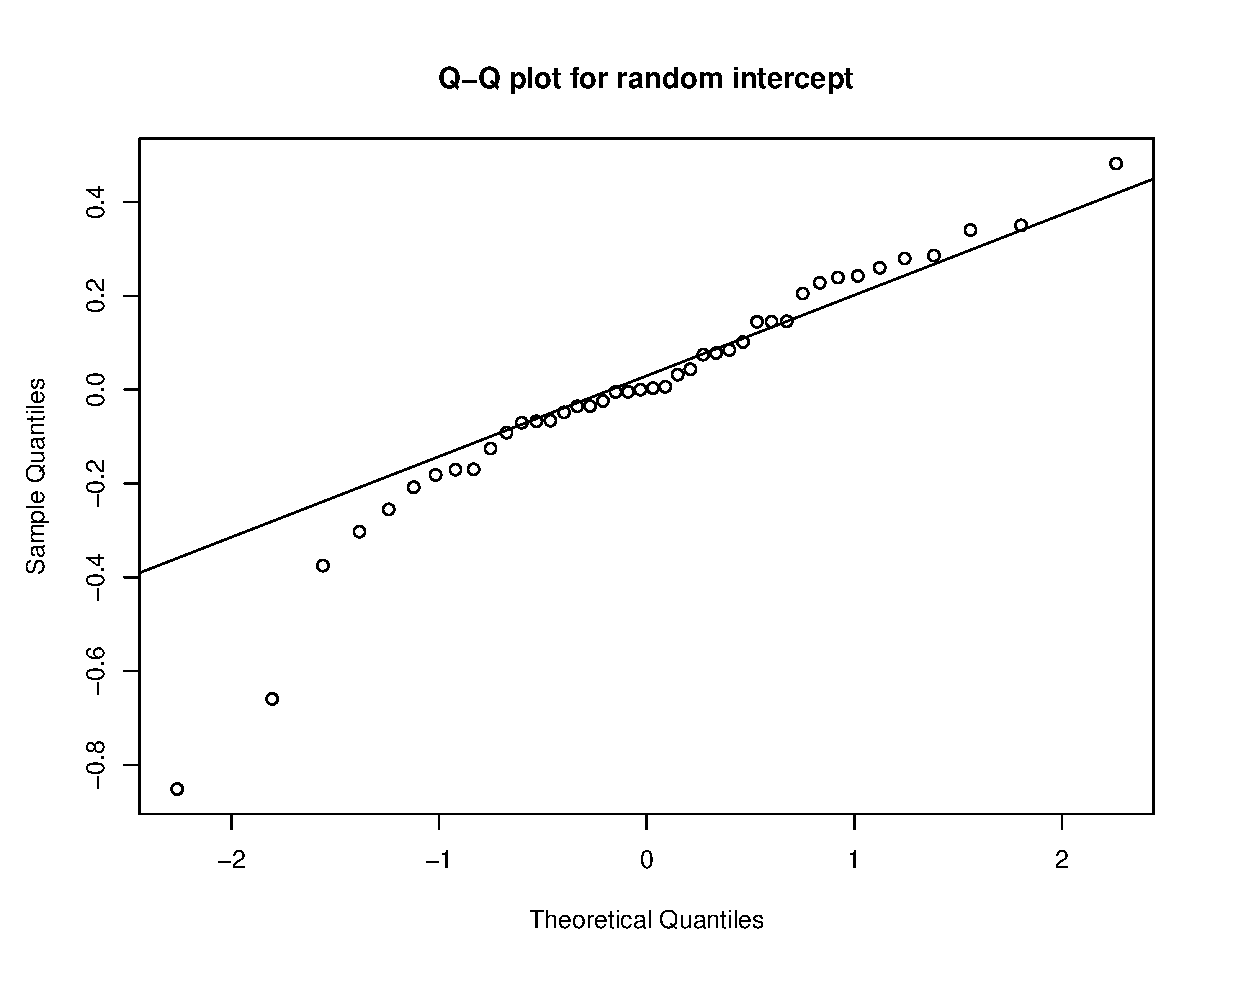
\includegraphics[width=0.50\textwidth]{../graphics/fig3.eps}  %\hspace{00cm}
\caption{ Q-Q plot for boat effect of the final GLMM model} %\vspace{1.05cm}
\label{fig3}
\end{figure}

\hspace{-6mm}\underline{Generalized additive mixed-effect model (GAMM) of binary wet weight }\\

A GAMM is just a GLMM in which part of the linear predictor is specified in terms of smooth functions of covariates. We fit a GAMM model considering $b$-splines of days1 and days2, and we used thin plate regression and cubic splines. Same as before, we first consider the model considering all variables and their interactions. We then dropping variables one by one that is insignificant and suggested by F-test. The final model includes the variables are days1, days2, painttype, LocID, days1:days2, days1:midrips, and days2:midTrips.
\begin{figure}
\centering
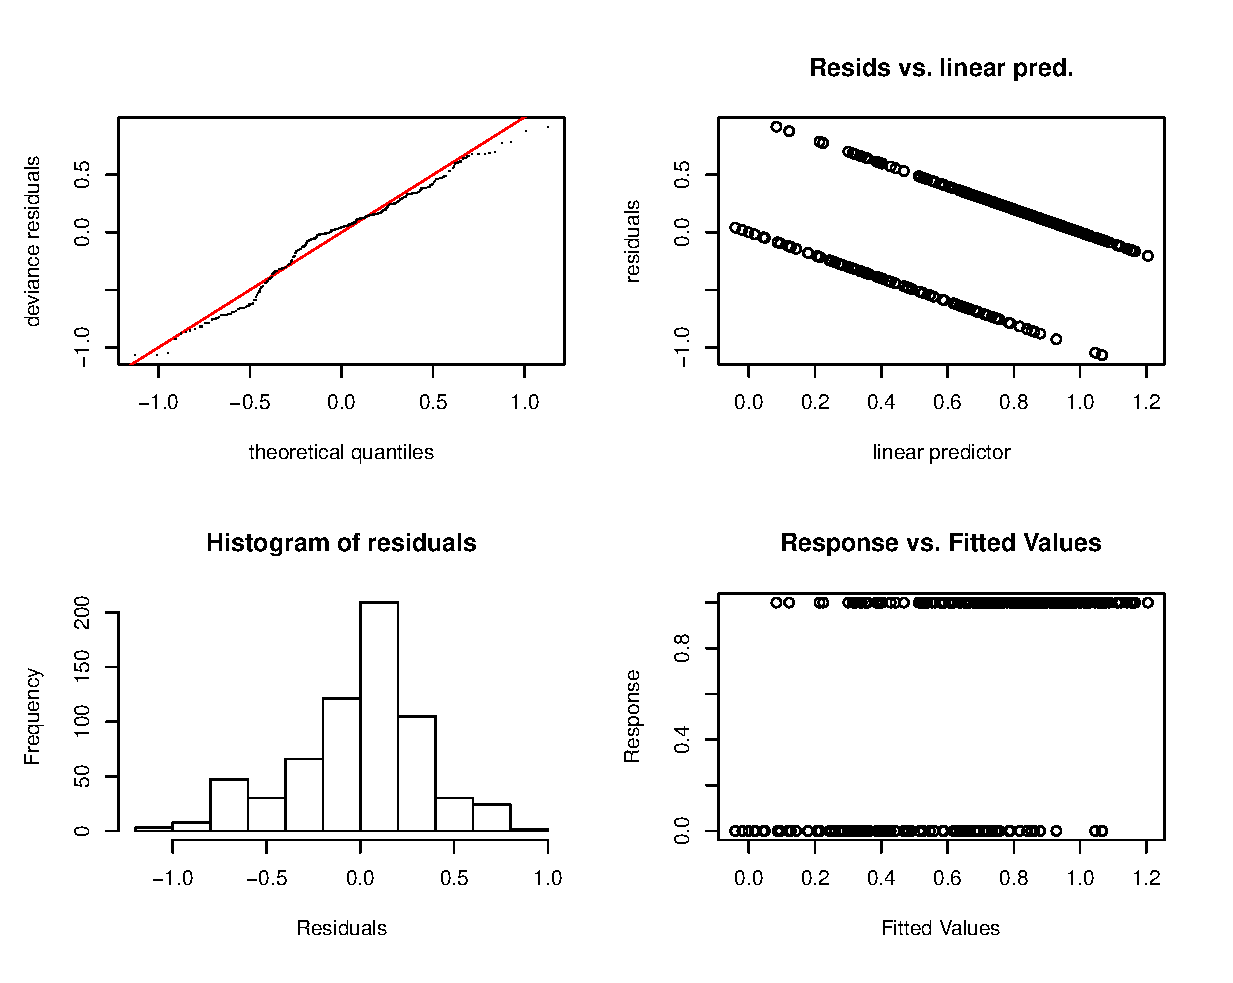
\includegraphics[width=0.60\textwidth]{../graphics/figgam.eps}  %\hspace{00cm}
\caption{Basic model checking plots for the final GAMM model.} %\vspace{1.05cm}
\label{figgam}
\end{figure}


gam.check is a routine that produces some basic residual plots, and a little further information about the success or otherwise of the fitting process (Wood, 2006). The plots produced for the final model are shown in Figure \ref{figgam}. gam.check of the model shows that Q-Q plot is very close to a straight line, suggesting the distributional assumption is reasonable.The residual plot suggests that variance is approximately constant. The Histogram of residual is approximately normal. The response against fitted values is reasonable. The residuals plot of the GAMM model are shown in Figure \ref{figgamglmer_res}. Thus nothing to be problematic and the final model is very logical in this scenario. The final GAMM is used to assess the independent effect of a variable on biomass. The results are presented in Table \ref{tab2}. The ANOVA table for the GAMM model is presented in Table \ref{tab3}. All the variables included in the model are significant.\\

\begin{figure}
\centering
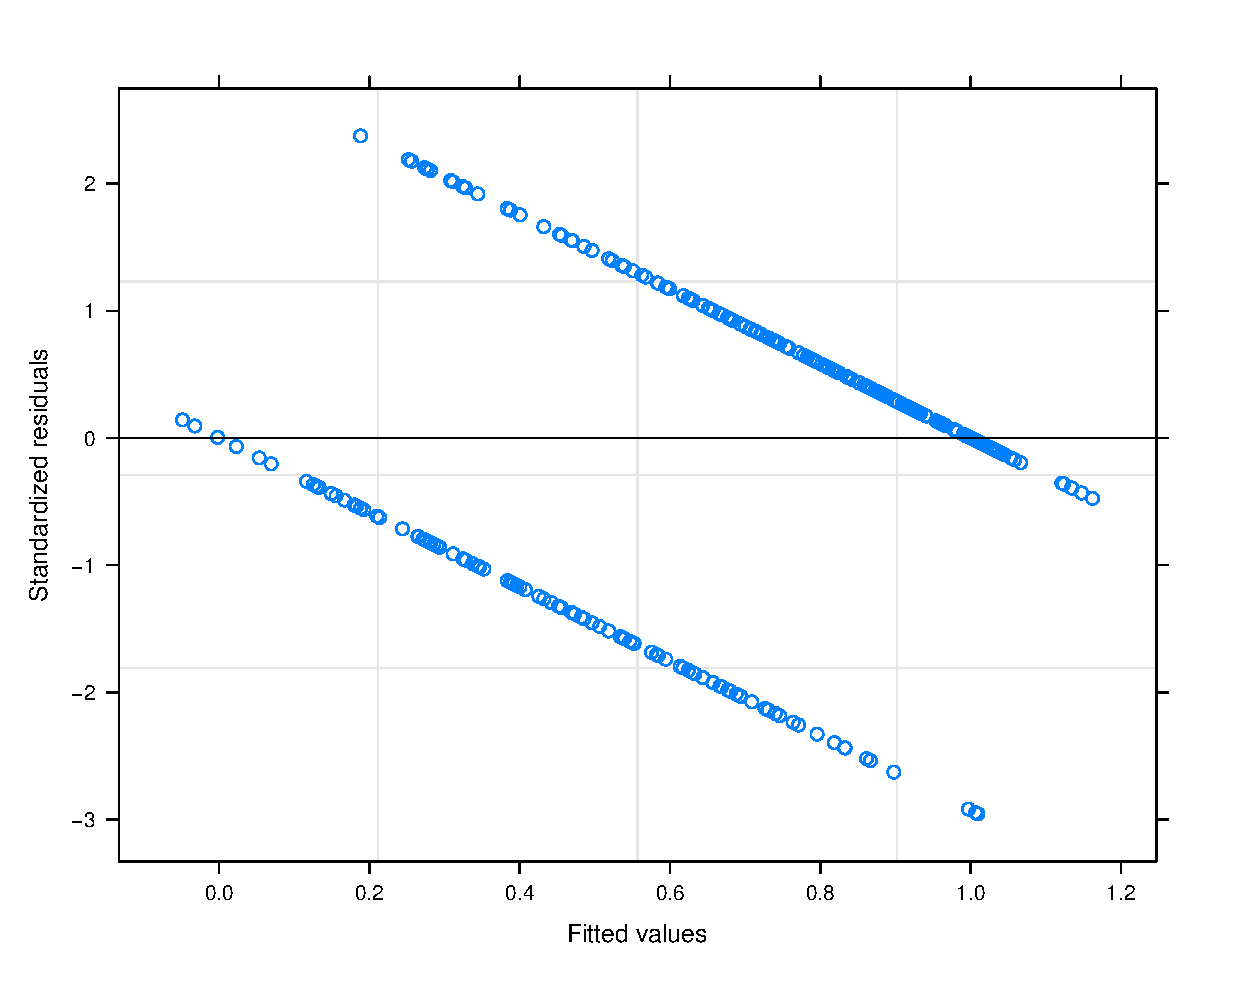
\includegraphics[width=0.50\textwidth]{../graphics/figgamglmer_res.eps}  %\hspace{00cm}
\caption{Residuals plot of the GAMM model.} %\vspace{1.05cm}
\label{figgamglmer_res}
\end{figure}


\begin{small}
\begin{table}
%\begin{center}
\caption{GAMM analysis for determining the determinants of biomass} \label{tab2}
\begin{tabular}{|c|c|c|c|c|} \hline

Parametric coefficients:            &Estimate &Std. Error &$t$ value &Pr$(>|t|$)\\
\hline
(Intercept)                    &9.945e-01  &6.198e-02  &16.046  &$<$ 2e-16 ***\\
paintTypeHard                  &3.387e-01  &1.198e-01  &2.827 &0.004854 ** \,\\
paintTypeSelf-polishing        &4.626e-01  &1.210e-01  &3.823 &0.000145 ***\\
factor(LocID)HAH               &2.745e-02  &6.123e-02  &0.448 &0.654100 \, \, \,\\
factor(LocID)HD               &-2.578e-01  &5.584e-02  &-4.617 &4.71e-06 ***\\
factor(LocID)HH               &-3.667e-02  &7.010e-02  &-0.523 &0.601085 \, \, \,\\
factor(LocID)HK               &-3.131e-01  &7.189e-02  &-4.355 &1.55e-05 ***\\
factor(LocID)HP               &-9.767e-02  &5.067e-02  &-1.927 &0.054369 . \, \, \\
factor(LocID)IB               &-1.950e-01  &4.131e-02  &-4.722 &2.88e-06 ***\\
factor(LocID)PB               &-1.314e-01  &6.019e-02  &-2.183 &0.029372 *\, \,\\
factor(LocID)PJ               &1.296e-02  &4.720e-02   &0.275 &0.783780 \, \, \,\\
days1:days2                   &-7.599e-06  &1.366e-06  &-5.564 &3.90e-08 ***\\
days1:midTrips                &-5.883e-05  &1.720e-05  &-3.421 &0.000663 ***\\
paintTypeHard:days2           &-6.441e-04  &6.169e-04  &-1.044 &0.296820 \, \, \,\\
paintTypeSelf-polishing:days2 &-1.727e-03  &3.885e-04  &-4.445 &1.04e-05 ***\\
\hline
Significance of smooth terms: &edf &Ref.df     &F  &$p$-value\\
\hline
s(days1)   &1   &1  &26.50  &3.53e-07 ***\\
s(days2)   &1   &1  &46.96 &1.73e-11 ***\\
\hline
\end{tabular}
\\

Signif. codes: \quad 0 �***� \quad 0.001 �**� \quad 0.01 �*� \quad 0.05 �.� \quad 0.1 \quad � � 1
%\end{center}
\end{table}
\end{small}


\begin{small}
\begin{table}
\centering
\caption{ANOVA Table for GAMM model of binary wet weight} \label{tab3}
\begin{tabular}{|c|c|c|c|} \hline
Parametric Terms:   &df      &F   &$p$-value\\
\hline
paintType           &2   &8.136   &0.000325\\
factor(LocID)       &8   &7.159   &4.27e-09\\
days1:days2         &1   &30.960  &3.90e-08\\
days1:midTrips      &1   &11.707  &0.000663\\
paintType:days2     &2   &9.975   &5.44e-05\\
\hline
Significance of smooth terms:   &Ref.df     &F  &p-value\\
\hline
s(days1)        &1 &26.50 &3.53e-07\\
s(days2)        &1 &46.96 &1.73e-11\\
\hline
\end{tabular}
\end{table}
\end{small}



\hspace{-6mm}\underline{Linear mixed-effect model (LMM) for non-zero biomass}\\

   Biomass collected from HA are all identically-sized quadrats, that is the area scraped was the same for each. Thus LMM analysis is performed on modeling the HA for volume. At first we consider modeling including all variables and then dropping variable that is insignificant and also suggests by both F-test and PB test. Continuing this process, we select the best model which includes variables are days2, midTrips, days1:midTrips and midTrips:painttype. The residual plot, Q-Q plot for residuals and Q-Q plot for random effect are shown in Figure \ref{figlmmres}, Figure \ref{figlmmqq} and Figure \ref{figlmmqqr} respectively.\\

 \begin{figure}
\centering
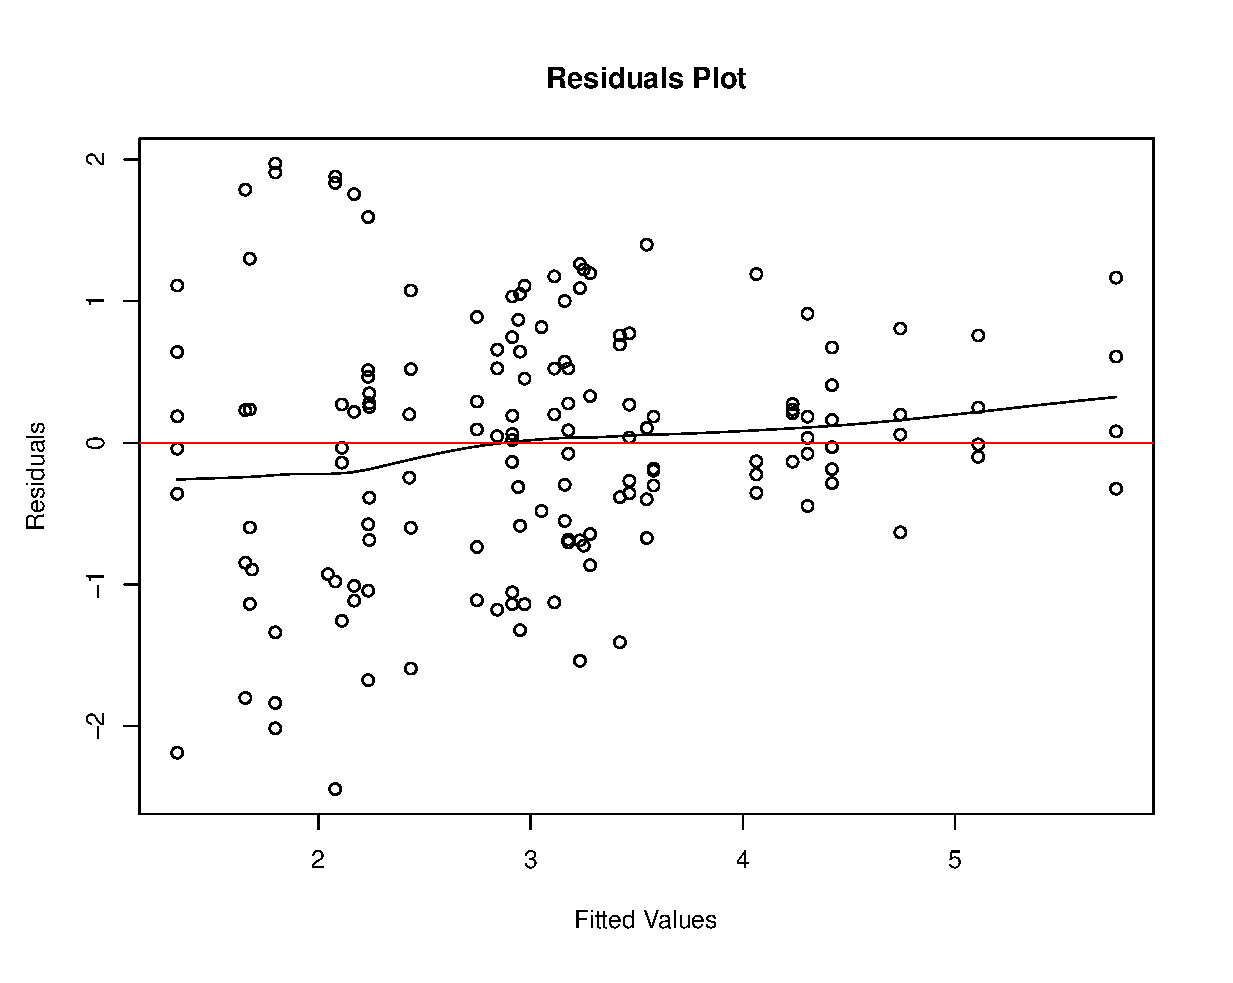
\includegraphics[width=0.50\textwidth]{../graphics/figlmmres.eps}  %\hspace{00cm}
\caption{Residual plot for LMM model} %\vspace{1.05cm}
\label{figlmmres}
\end{figure}



Variance-adjusted, outermost residuals have approximately constant variance as the residuals do not have any relationship. There are is no curved pattern that indicates that the residual are normally distributed. There are no substantial outliers. Thus it can be said that LMM model fits the data reasonable well. The Q-Q plot for residuals follows approximately in the line, that means two distributions agree after linearly transforming the values. However, Q-Q plot for for random effect slightly differ from straight line but more reasonable than the full model, suggesting the model is appropriate. The summary results of the final LMM model are presented in Table \ref{tablmmsum}. The Analysis of variance table for LMM model are given in Table \ref{tablmmanova}.

\begin{figure}
\centering
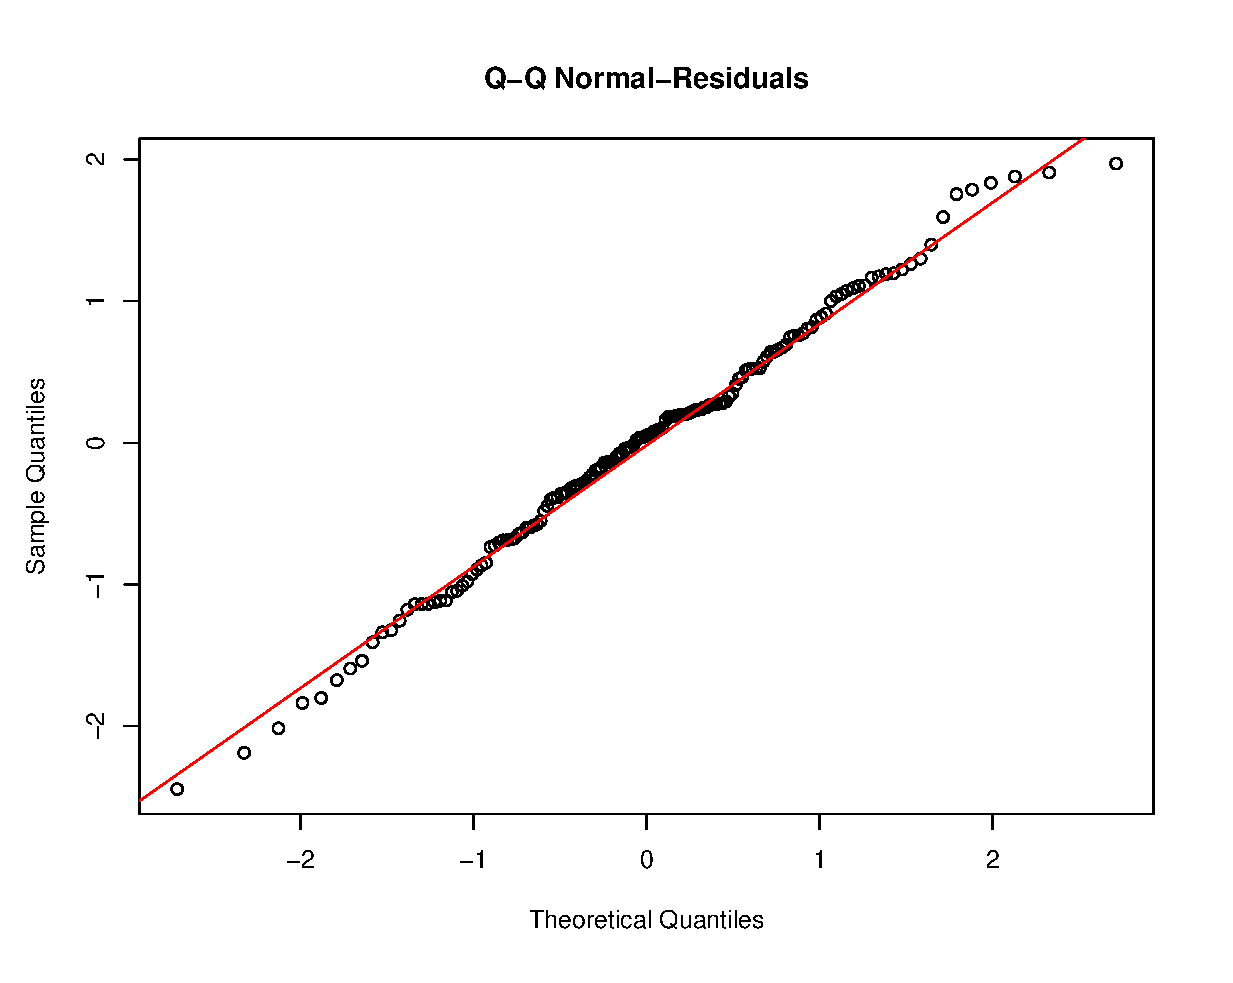
\includegraphics[width=0.50\textwidth]{../graphics/figlmmqq.eps}  %\hspace{00cm}
\caption{Q-Q plot for residuals of LMM model} %\vspace{1.05cm}
\label{figlmmqq}
\end{figure}



\begin{figure}
\centering
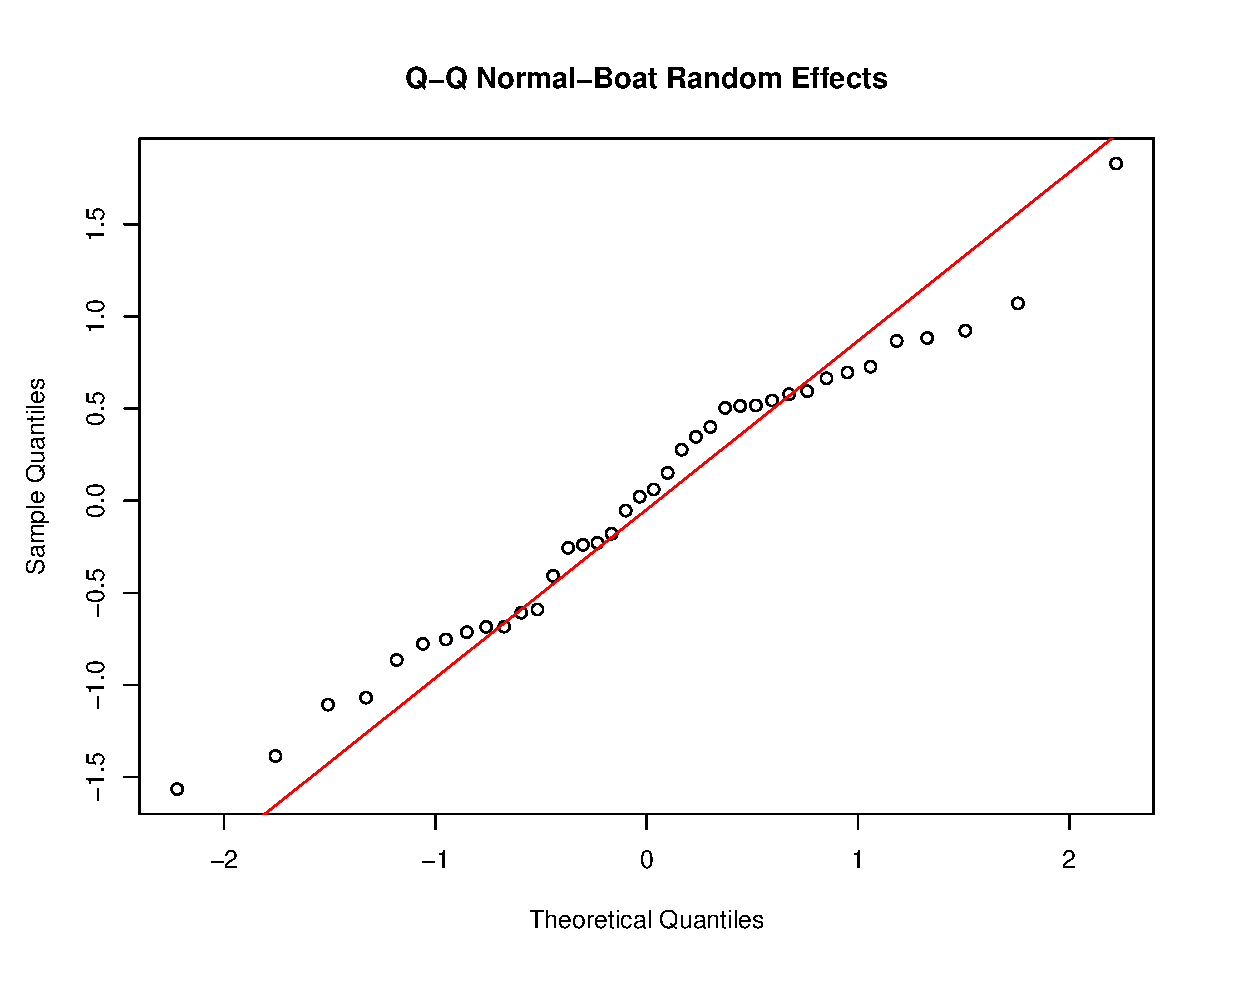
\includegraphics[width=0.50\textwidth]{../graphics/figlmmqqr.eps}  %\hspace{00cm}
\caption{Q-Q plot for boat random effect of LMM model} %\vspace{1.05cm}
\label{figlmmqqr}
\end{figure}




\begin{small}
\begin{table}
%\begin{center}
\caption{Parameter estimates of LMM model (all vessels) of hull biofouling wet weight} \label{tablmmsum}
\begin{tabular}{|c|c|c|c|c|c|} \hline
Fixed effects:                     &Value       &Std.Error      &DF     &$t$-value  &$p$-value\\
\hline
(Intercept)                       &2.6115591     &0.31568390     &112    &8.272703   &0.0000\\
days2                             &0.0037833     &0.00105958     &32     &3.570554   &0.0012\\
midTrips                          &-0.0287641    &0.01219281      &32      &-2.359105   &0.0246\\
midTrips:days1                    &0.0000059     &0.00006629      &32      &0.088313    &0.9302\\
midTrips:paintTypeHard            &0.0261187     &0.01201783      &32      &2.173327    &0.0373\\
midTrips:paintTypeSelf-polishing  &0.0201287     &0.01140736      &32      &1.764534    &0.0872\\
\hline
\end{tabular}
\end{table}
\end{small}





\begin{small}
\begin{table}
\centering
\caption{ANOVA table for LMM model} \label{tablmmanova}
\begin{tabular}{|c|c|c|c|c|} \hline
  \quad              &numDF &denDF  &$F$-value &$p$-value\\
  \hline
(Intercept)            &1   &112 &384.4098  &$<$.0001\\
days2                  &1    &32   &6.4723  &0.0160\\
midTrips               &1    &32   &5.4299  &0.0263\\
midTrips:days1         &1    &32   &0.6437  &0.4283\\
midTrips:paintType     &2    &32   &2.4649  &0.1010\\
\hline
\end{tabular}
\end{table}
\end{small}

Days2 is strongly significant, whereas midTrips are significant at 5\% level of significance. PaintType itself
is not a significant but it�s interaction with midTrips are statistically significant. If the vessel is not
cleaned one day, then the log of the wet weight is increased by .004 grams given an ablative antifouling paint is used
and other variables are constant. On the other hand, similar if ablative antifouling paint is used the log of the wet
weight is decreased by .029 grams, if median number of trips is increased by one day when other variables are constant.
paintType influence the effect of vessel activity on the log of the wet weight of biofouling. On an average midTrips, hard
paint is significant on fouling biomass compared to ablative paint.\\



\hspace{-6mm}\underline{Generalized additive mixed-effect model (GAMM) for non-zero biomass}\\

We fit a GAMM model for non-zero biomass collected from only HA. We consider smooths of days1 and days2 and parametric terms of other variables.
Same as before, we select a best GAMM model by dropping variable one by one using F-test. The final model includes the variables are days2, midTrips, days1:paintType, days2:midTrips, days2:paintType and midTrips:paintType.


 \begin{figure}
\centering
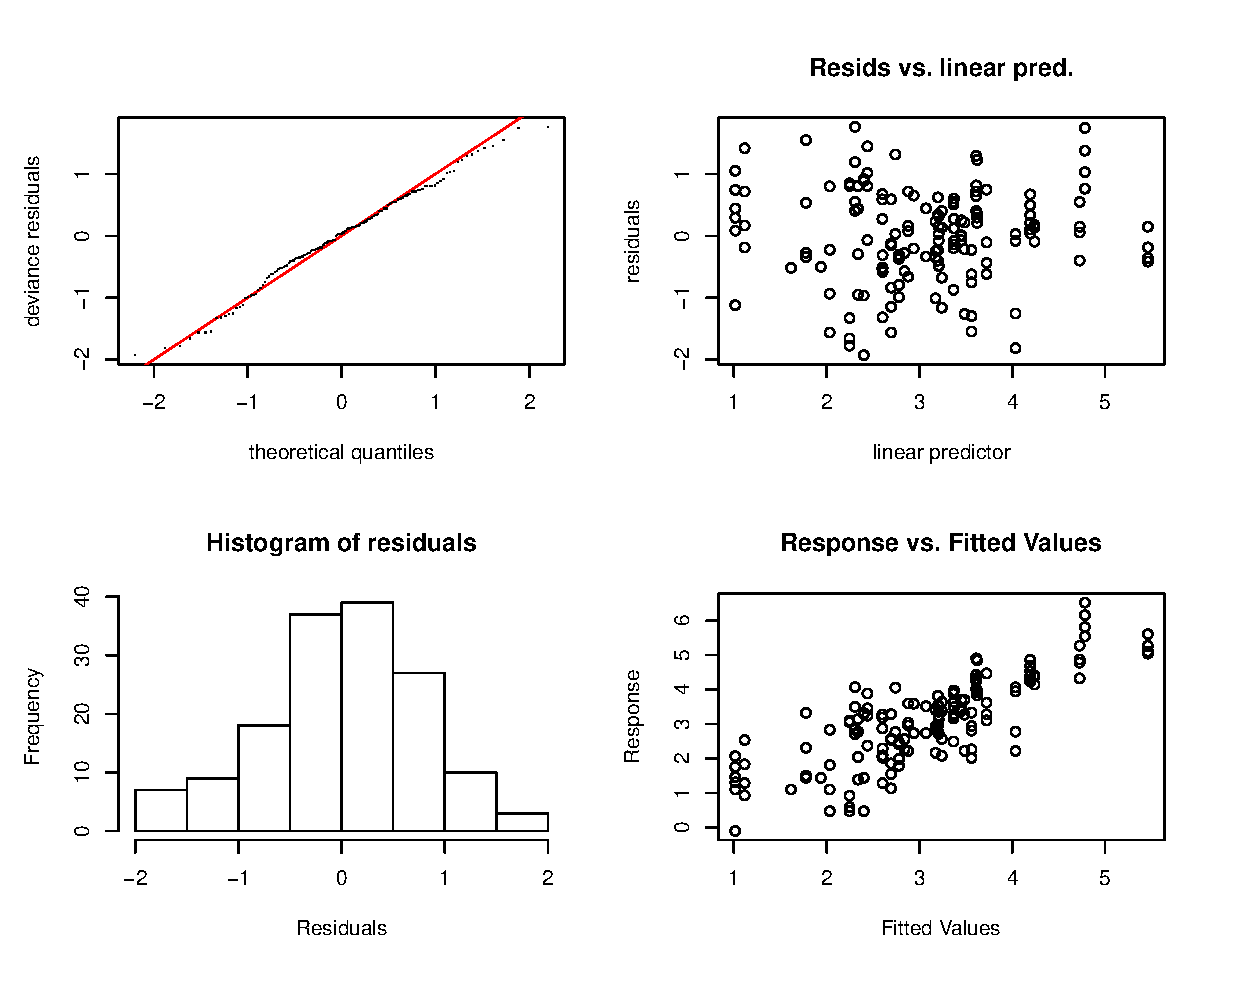
\includegraphics[width=0.60\textwidth]{../graphics/figgamha.eps}  %\hspace{00cm}
\caption{Basic model checking plots for the GAMM model of hull biofouling wet weight.} %\vspace{1.05cm}
\label{figgamha}
\end{figure}


gam.check of the model in Figure \ref{figgamha} shows that Q-Q plot is very close to a straight line, suggesting the distributional assumption is reasonable. The residual plot suggests that variance is approximately constant as mean increases. The Histogram of residuals is approximately
consistent with normality. The plot of response against fitted values shows a positive relationship with a moderate scatter. The residual plot for the GAMM are given in Figure \ref{figgamha_res}. The residual plots very good and thus model is very reasonable. The summary results and the ANOVA are presented in Table \ref{tabgamha} and Table \ref{tabgamanovaha} respectively.


 \begin{figure}
\centering
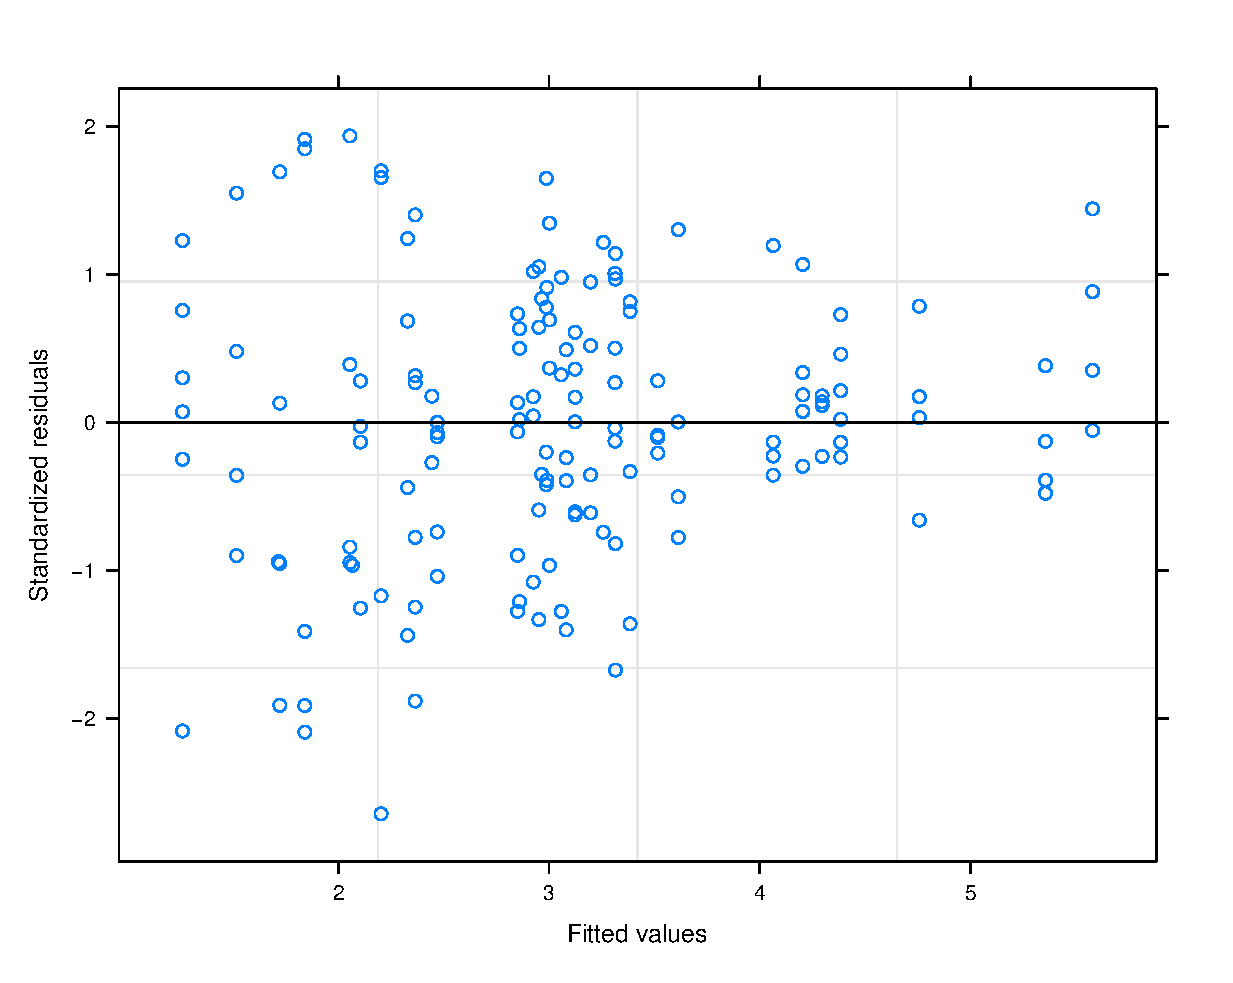
\includegraphics[width=0.60\textwidth]{../graphics/figgamha_res.eps}  %\hspace{00cm}
\caption{Residual plot for the GAMM model of hull biofouling wet weight.} %\vspace{1.05cm}
\label{figgamha_res}
\end{figure}


\begin{small}
\begin{table}
%\begin{center}
\caption{Parameter estimates of GAMM model (all vessels) of hull biofouling wet weight} \label{tabgamha}
\begin{tabular}{|c|c|c|c|c|} \hline
Parametric coefficients:          &Estimate &Std. Error &$t$ value &Pr($>$|t|)\\
\hline
(Intercept)                       &3.858e+00  &2.334e-01  &16.529  &$<$ 2e-16 ***\\
midTrips                         &-5.239e-02  &1.210e-02  &-4.331 &2.86e-05 ***\\
days1:paintTypeAblative           &3.052e-03  &1.402e-03   &2.177 &0.031228 *\\
days1:paintTypeHard              &-8.834e-04  &2.427e-03  &-0.364 &0.716442\\
days1:paintTypeSelf-polishing     &2.696e-03  &1.852e-03   &1.456 &0.147749\\
midTrips:days2                    &3.023e-05  &2.274e-05   &1.329 &0.185961\\
paintTypeHard:days2              &-3.028e-03  &2.986e-03  &-1.014 &0.312363\\
paintTypeSelf-polishing:days2    &-3.927e-03  &1.291e-03  &-3.041 &0.002828 **\\
midTrips:paintTypeHard            &4.482e-02  &1.148e-02   &3.903 &0.000149 ***\\
midTrips:paintTypeSelf-polishing  &3.775e-02  &9.687e-03   &3.897 &0.000152 ***\\
\hline
Significance of smooth terms:     &edf &Ref.df     &F  &$p$-value\\
\hline
s(days2) &3.485  &3.485 &10.67 &6.03e-07 ***\\
\hline
\end{tabular}

Signif. codes:  0 �***� 0.001 �**� 0.01 �*� 0.05 �.� 0.1 � � 1
\end{table}
\end{small}





\begin{small}
\begin{table}
\centering
%\begin{center}
\caption{ANOVA table for GAMM model of non-zero biomass} \label{tabgamanovaha}
\begin{tabular}{|c|c|c|c|c|} \hline
Parametric Terms:   &df      &F  &$p$-value\\
\hline
midTrips            &1 &18.754 &2.86e-05\\
days1:paintType     &3  &2.355 &0.074717\\
midTrips:days2      &1  &1.767 &0.185961\\
paintType:days2     &2  &4.684 &0.010782\\
midTrips:paintType  &2  &8.602 &0.000303\\
\hline
Approximate significance of smooth terms:    &Ref.df     &F  &$p$-value\\
\hline
s(days2) &3.485 &10.67 &6.03e-07\\
\hline
\end{tabular}
\end{table}
\end{small}


Generalized additive mixed-effect model (GAMM) of hull biofouling wet weight suggests that smooth term days2 and midTrips are strongly significant.
However the interaction term midTrips:paintType are also significant whereas days2:midTrips are significant at 5\% level of significance.






\end{document}
